\documentclass[12pt]{scrartcl}
\title{Assignment 3\\ Design Thinking\\ Sketches and Wireframes}
\author{\textbf{Flow Overstack Team}\\ Cesana Filippo\\ Folli Gary\\ Hartmann Kathrin\\ Rodolfo Masera Tommaso\\ Stucchi Jacopo\\ Taillefert Stefano}
\date{}
\setlength{\parindent}{0pt}

\usepackage{graphicx}
\usepackage{float}
\usepackage[margin = 3cm]{geometry}


\begin{document}

\maketitle

\tableofcontents

\newpage


\section{Introduction}

	%Write a brief introduction referring back to your project and it basic concepts.
	
	Our app belongs to those apps who focus on the social side of technology.  The main idea revolves around the concept of learning new information about the life of important historical people through the use of the smartphone camera. The user will take a picture of herself or a friend - more generally of a human being - and the app will associate that face with the profile of an important people from the present and from the past. The app social side comes into play just after the picture, when the user decides whether to share the discovered profile on the app feed, where every people connected with the user (her friends) share their new discoveries.\\
	
	Since we aim to create an entertaining, social, and interactive way of learning, our persona is fundamentally ageless. Everyone who is able to read and willing to learn represents a possible user of our app - which for its focus on important people we named it V.I.P. While we suppose that learning may enjoyable for everyone, independently from age and cultural background, we also recognize a special interest in subvert the conception that the new young generation may have about VIP - especially young people around the age of twelve, for they are at the beginning of their education and they may still lack the critical thinking tools which are required to understand the artificial construction behind certain online profiles which are successful in terms of likes and followers, such as those appearing on Instagram and Facebook. Our best hopes for this app are therefore shaped by a desire to redirect the vision of VIP which the new young generation may have. By sharing profiles such as those of Leonardo Da Vinci e Nikola Tesla, which gained fame by changing culture, history, and technology, instead of representing a collection of materialistic and ephemeral signs as most of the successful VIP on the social media tend to appear, we follow this goal.\\
  
	We firstly interrogated ourselves about possible funny ways to learn.  We already had in mind an interactive approach, for it is generally perceived as more entertaining. After having interview some young girls and boys of the Elvetico school, and merging together the aforementioned concepts, we concluded that a photography associated with the face of a friend, leading to a connection with an actual VIP, may have been the right path to follow. 


\section{Persona}

	% Describe briefly your design persona as distilled from the analysis of data gathered during Contextual Inquiry.
	
	The first task we went through was to summarize the interviews we conducted and extract meaningful data from all the kids' 
	answers to construct a user model for our application. The result is Kiddo, our design persona. Let us introduce him:\\
	
	Kiddo is the average 12-years-old, goes to middle school and loves spending time on his smartphone. He uses it mainly for 
	entertainment purposes, following his favorite youtubers and idols on social media, listening to music and chatting with his on- 
	and offline friends. Although its high affinity to his electronic device, our boy knows that he shouldn't exceed the usage limits 
	imposed by his parents and is well-aware that mobile phone addiction is just around the corner. For that reason, he doesn't
	stay on his phone for more than a couple of hours a day.\\
	
	He follows people like Footballo Socceri, the millionaire football player who likes to party and buy fast cars; 
	Trappino Trappisti, a rapper who rose to fame after punching a man on the street and whose songs are mainly violence-themed;
	Thotella DeThot, a TV showgirl widely known for her osé selfies posted on Instagram; and many others. Despite being interested 
	in their luxurious and cool lifestyle, Kiddo knows that they are not a good role model to follow; he is rather inspired by people
	who did something good for science, played a role in the history of humanity or left an important message for the future
	generations.\\
	
	Our persona doesn't dislike school, but he finds the ``classic" way of studying quite boring, bent over a textbook trying to memorize 
	dates and facts that he will forget in a couple of days anyway. In class, he often dreams of being somewhere else, learning 
	about something that \textit{really} amazes him. Kiddo thinks that there should be other ways of learning and that it should be
	more interactive.\\	
	
	\begin{figure}[H]
        		\centering
       		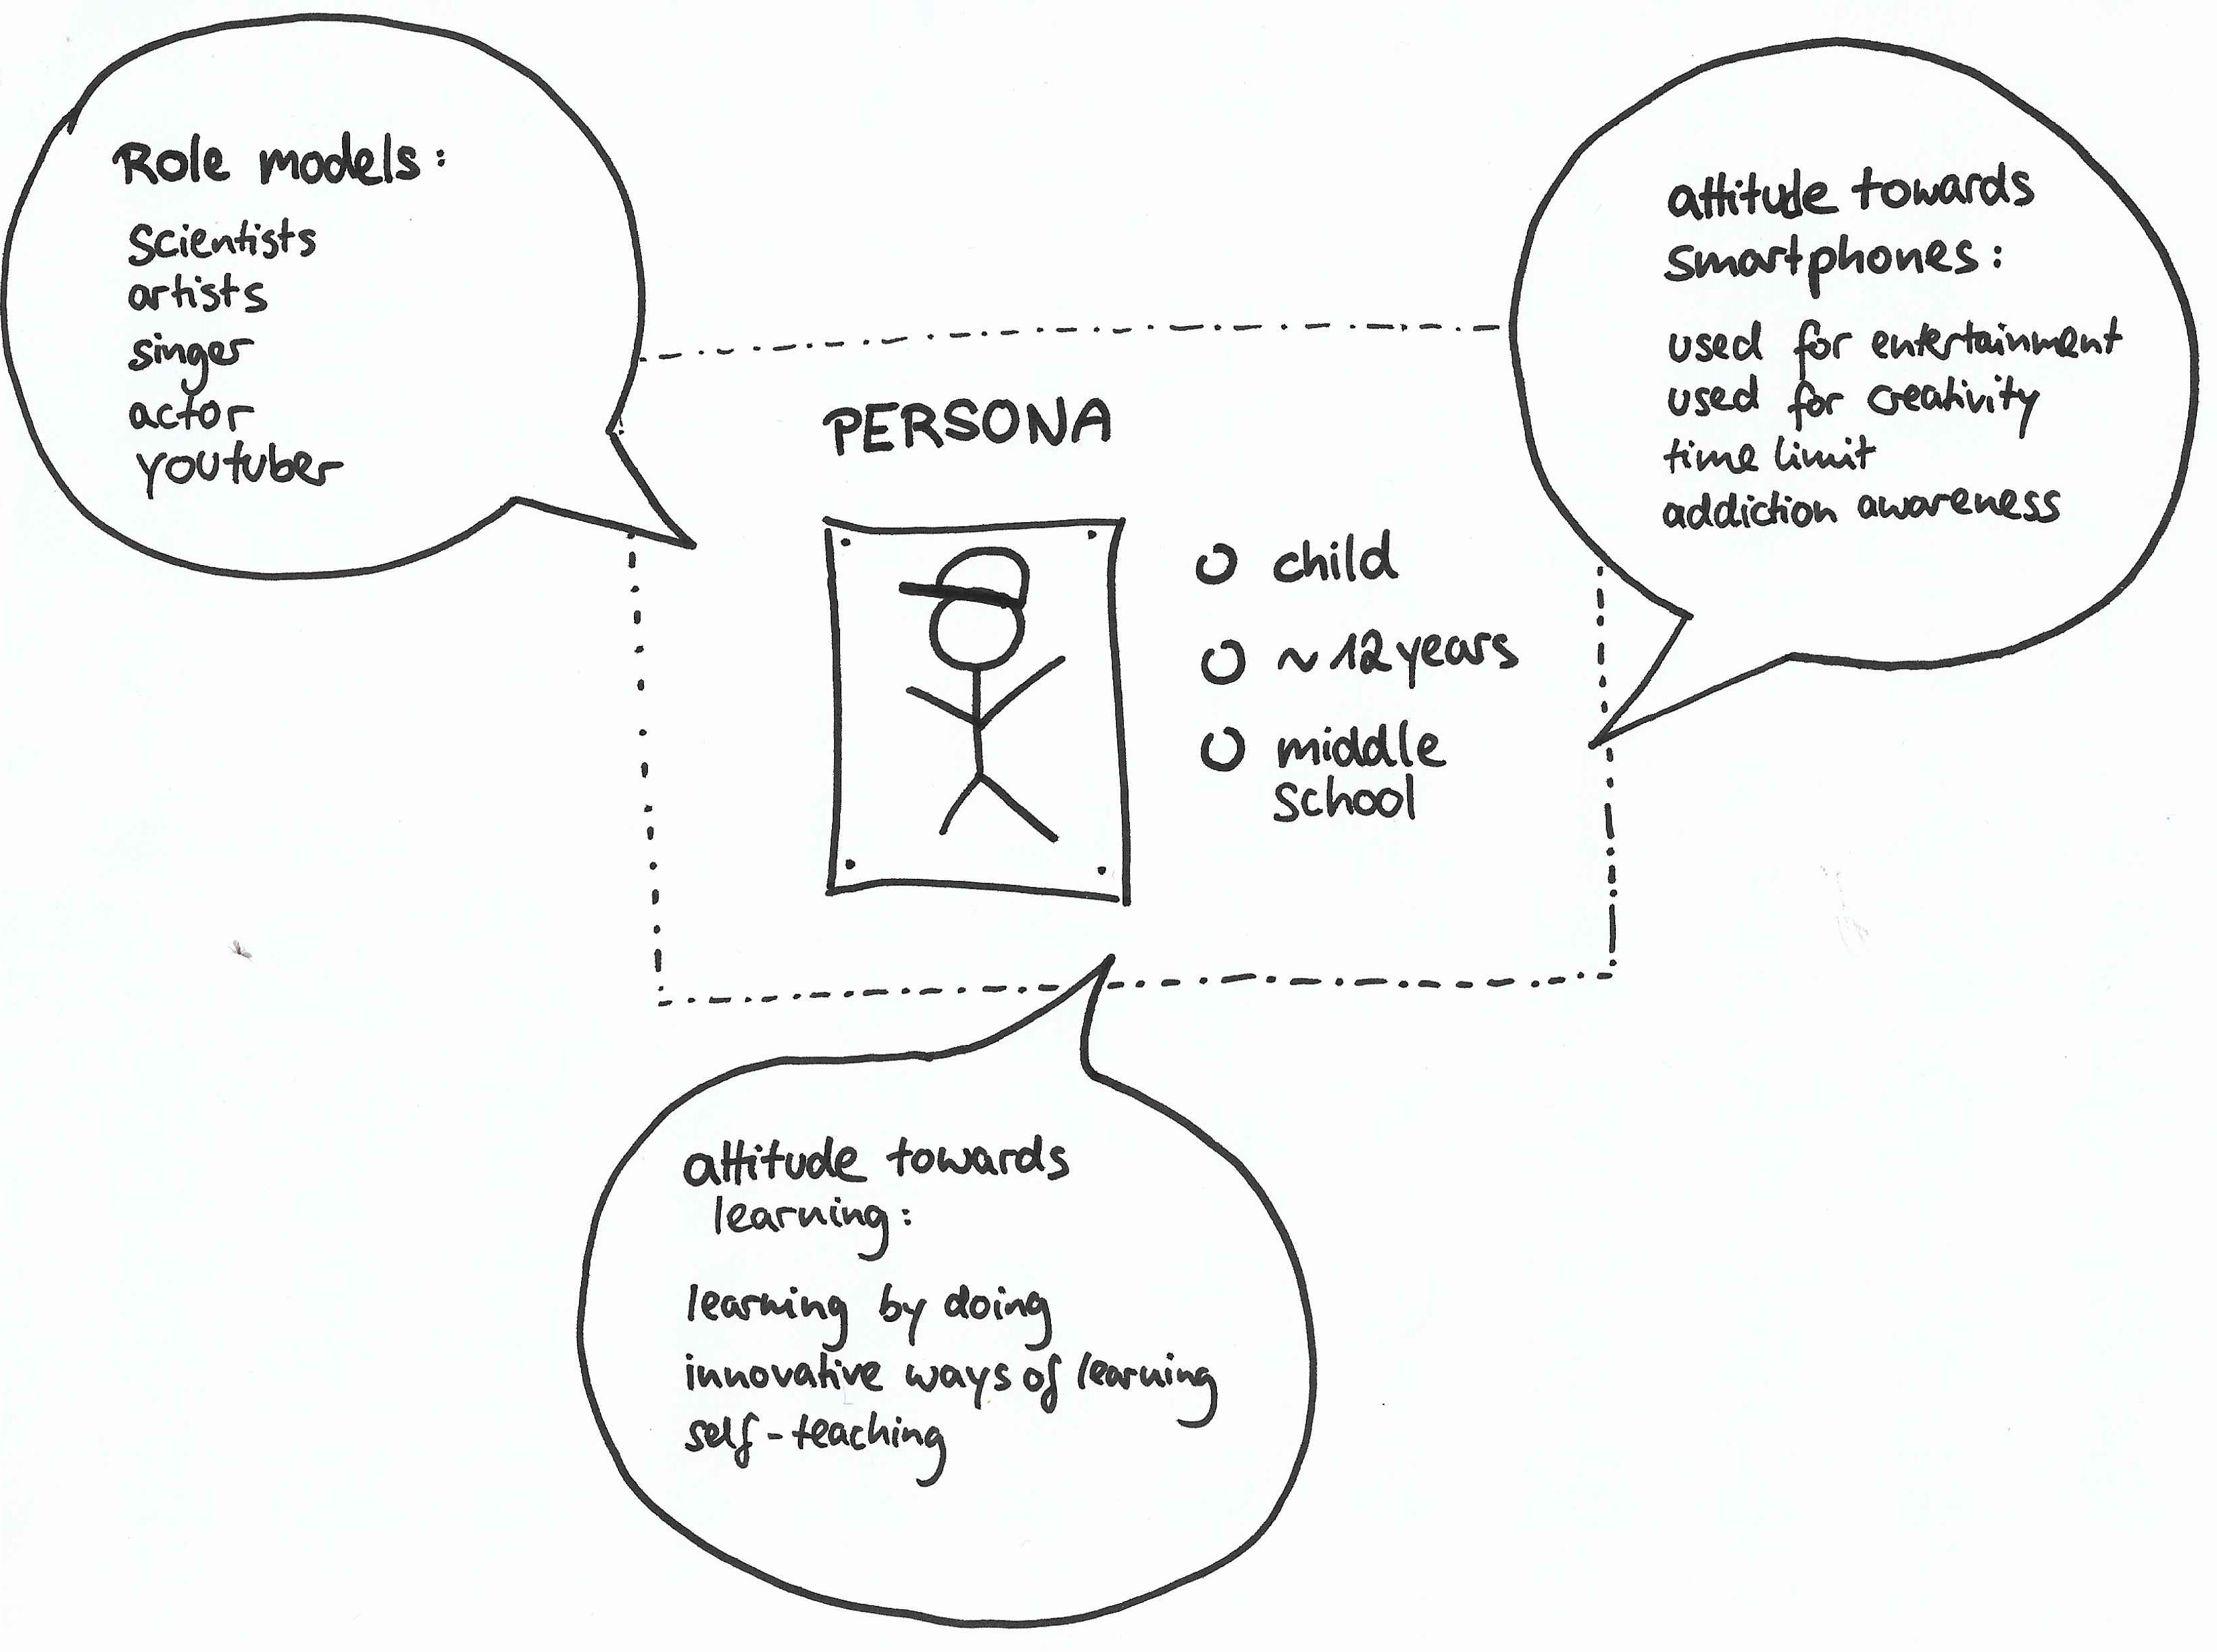
\includegraphics[width=\textwidth]{../images/persona2.jpg}
       		\caption{Our persona draft}
        		\label{persona1}
	\end{figure}
	

\section{Ideation and sketching}

	Before being able to sketch a storyboard and a wireframe we had to identify the persona we 
	were going to design the application for. With that in mind we went over the data we gathered
	through the interviews.\\
	
	The ideation followed right after. As we reviewed our information we came up with and sketched 
	some storyboards depicting a possible situation which our users may find themselves in. 
	For instance, you could imagine a child wondering what they would want to be when they grow
	up; in such a situation our application may help a kid clear their mind or come up with something
	new they would want to check out.\\
	
	Other than the storyboards, we sketched the skeleton of a possible wireframe, which will be
	covered in more detail in its own section, but the main idea behind it is to make it, firstly,
	simple and intuitive. We do not wish for our users to feel overwhelmed or lost because of
	many unclear features; because of this, at this point in time, we opted for few and easy to
	understand mechanics, such as a feed, a camera button and menus for a personal profile and
	settings.\\
	
	To wrap it up, ideation and sketching took shape together as they complement each other for
	a successful early design. The ideation was a necessary step to sketch our ideas since we
	could not have drawn anything without first coming up with something to draw ourselves.
	Reviewing our data was the fundamental point of this step as we could not have proceeded
	otherwise.

\section{Workspace and materials}

	% Describe your workspace and the materials you used.
	
	Our workspace is basically a desk in the Informatics building, either in a class room or in the open space. The desk is mostly rectangular 
	but we sit around it as if it was King Arthur's round table. In that way, everybody can contribute his creative ideas. For drawing sketches, 
	designing storyboards and creating drafts, we go easy and plain: Paper and black pens are our fundamental material. 
	Colours are only used for highlighting and structuring.\\
	
	Apart from that, we use the walls in our class room to draft larger sketches. Drawing on the wall enables us from time to time to explain 
	complex ideas in a very easy way to our group members.\\
	
	For the prototype we used the program ``Balsamiq" that lets us create sketchy wireframes in a convenient and easy way.
	
\section{Photos}

	% If appropriate, show photos of your team at work.
	
	\begin{figure}[H]
        		\centering
       		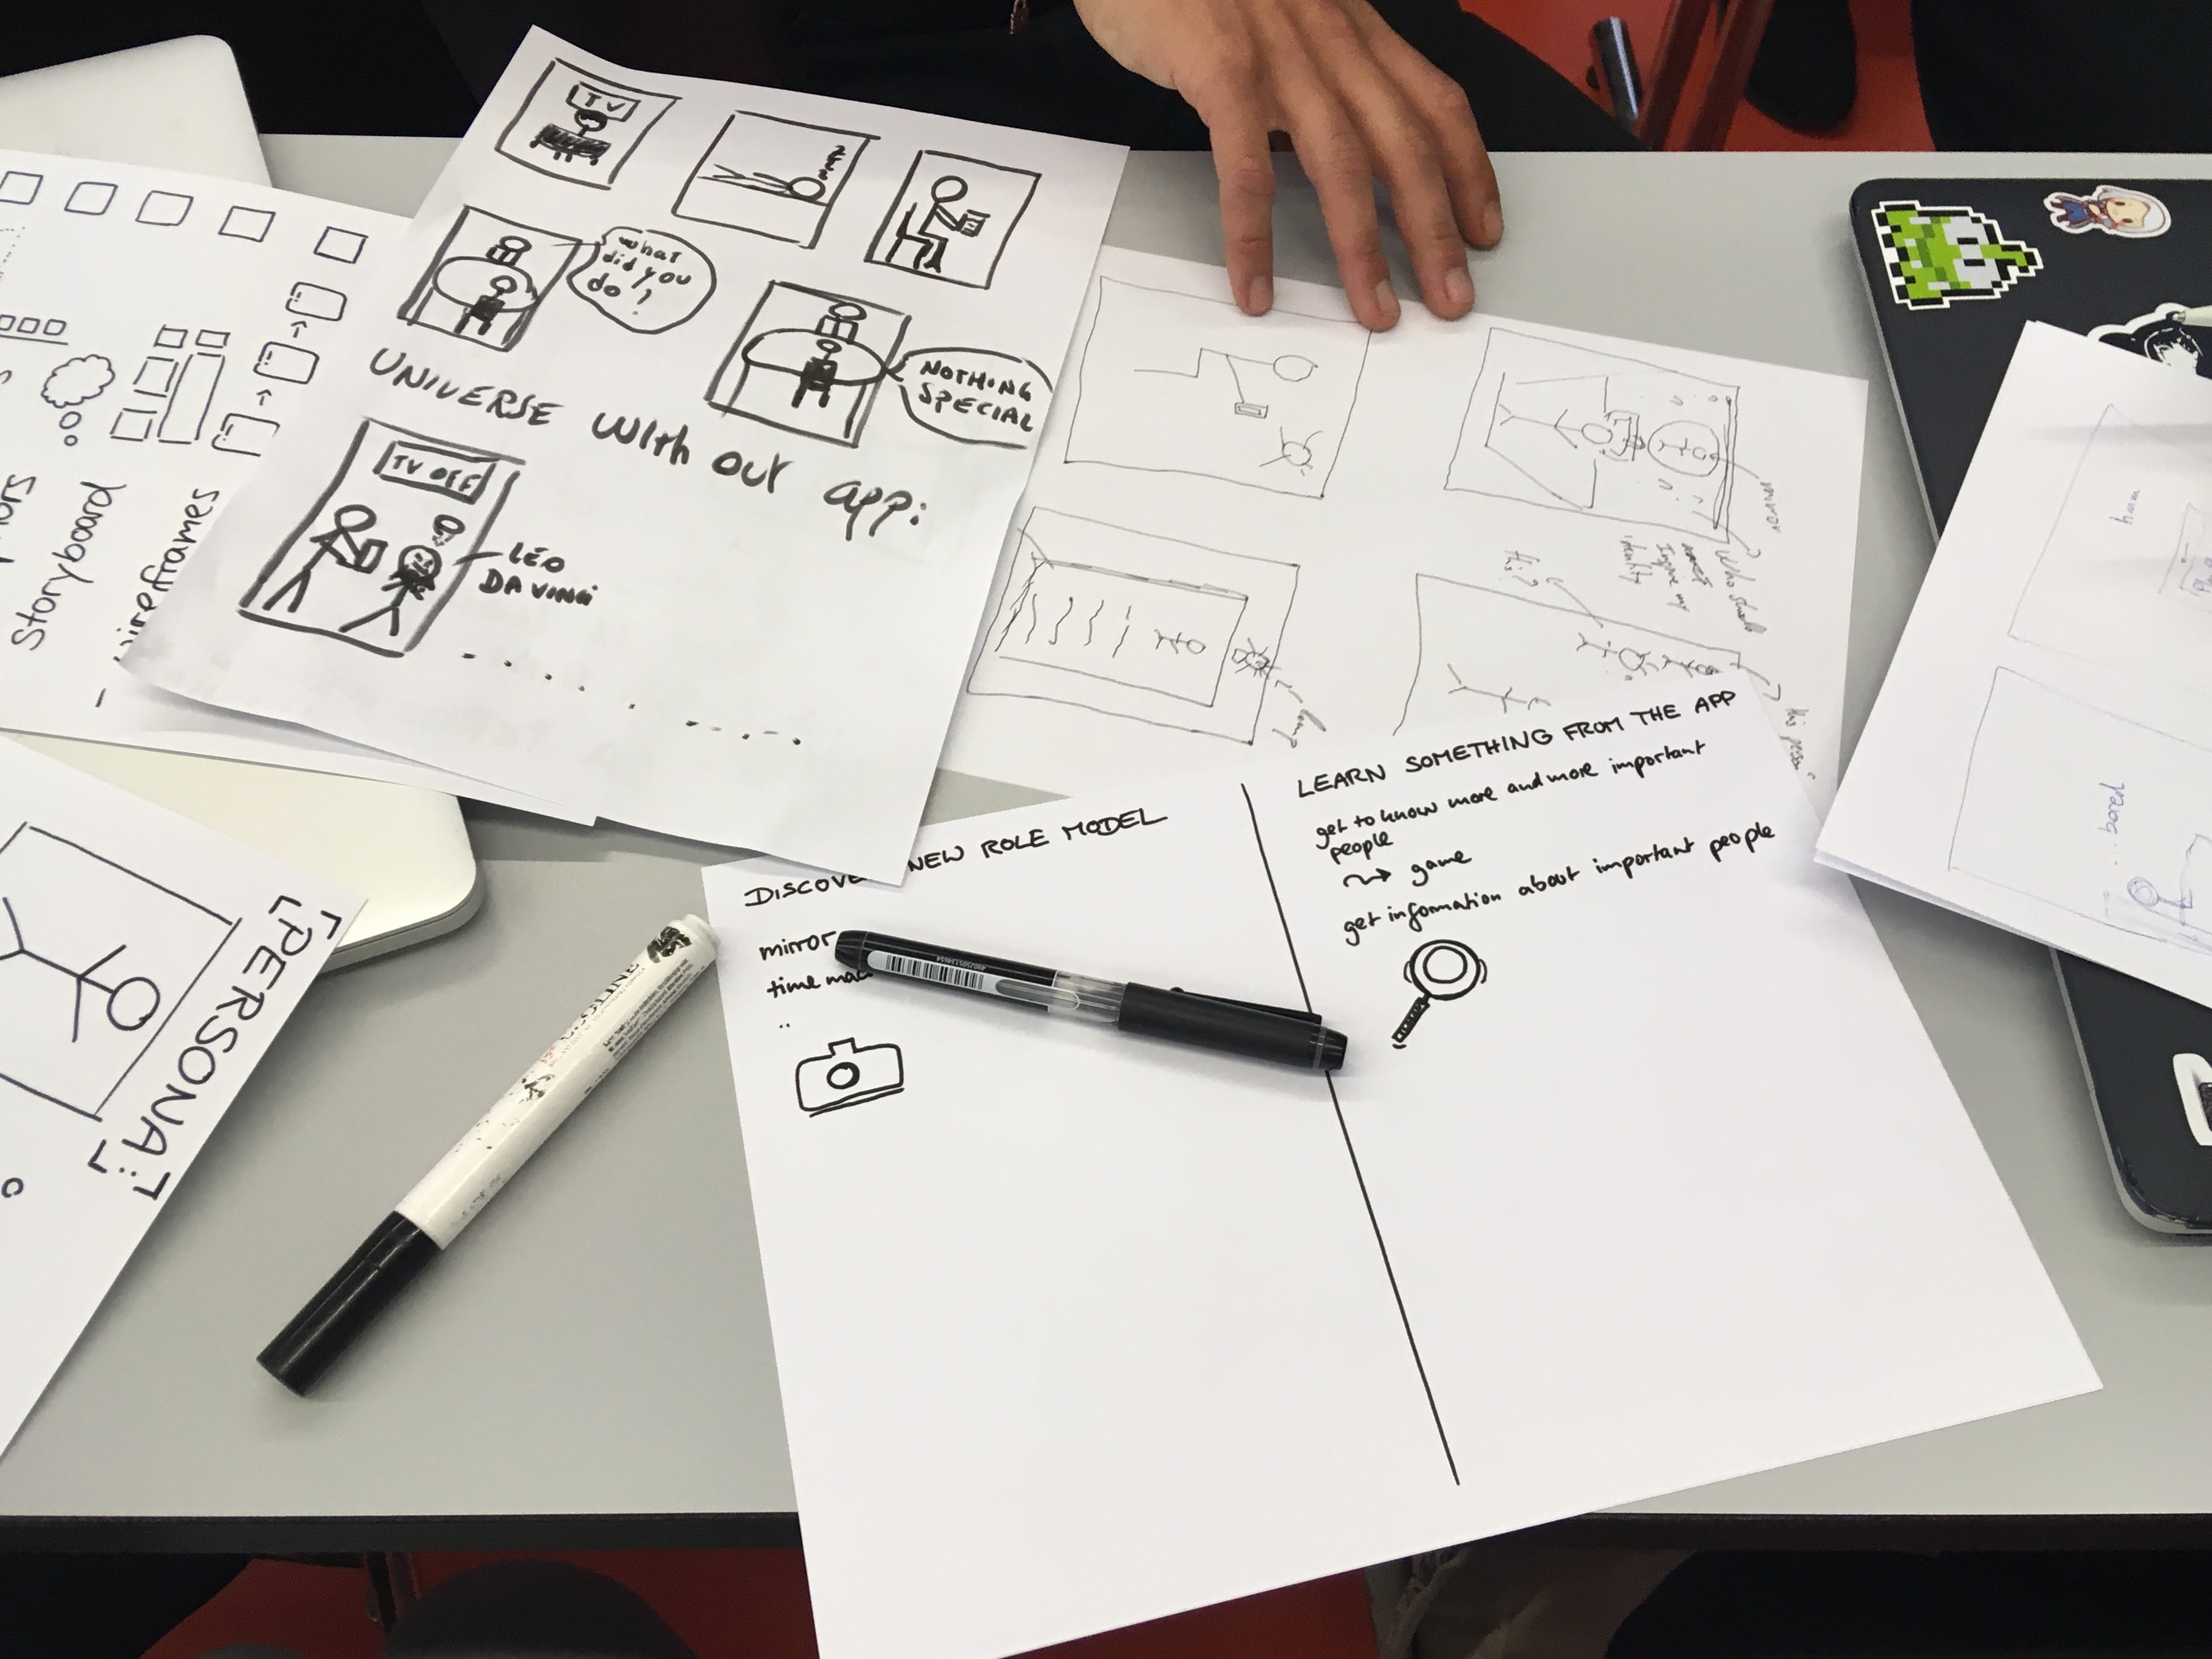
\includegraphics[width=\textwidth]{../images/group1.jpg}
       		\caption{Our creative sketching workspace}
        		\label{group1}
	\end{figure}
	
	\begin{figure}[H]
        		\centering
       		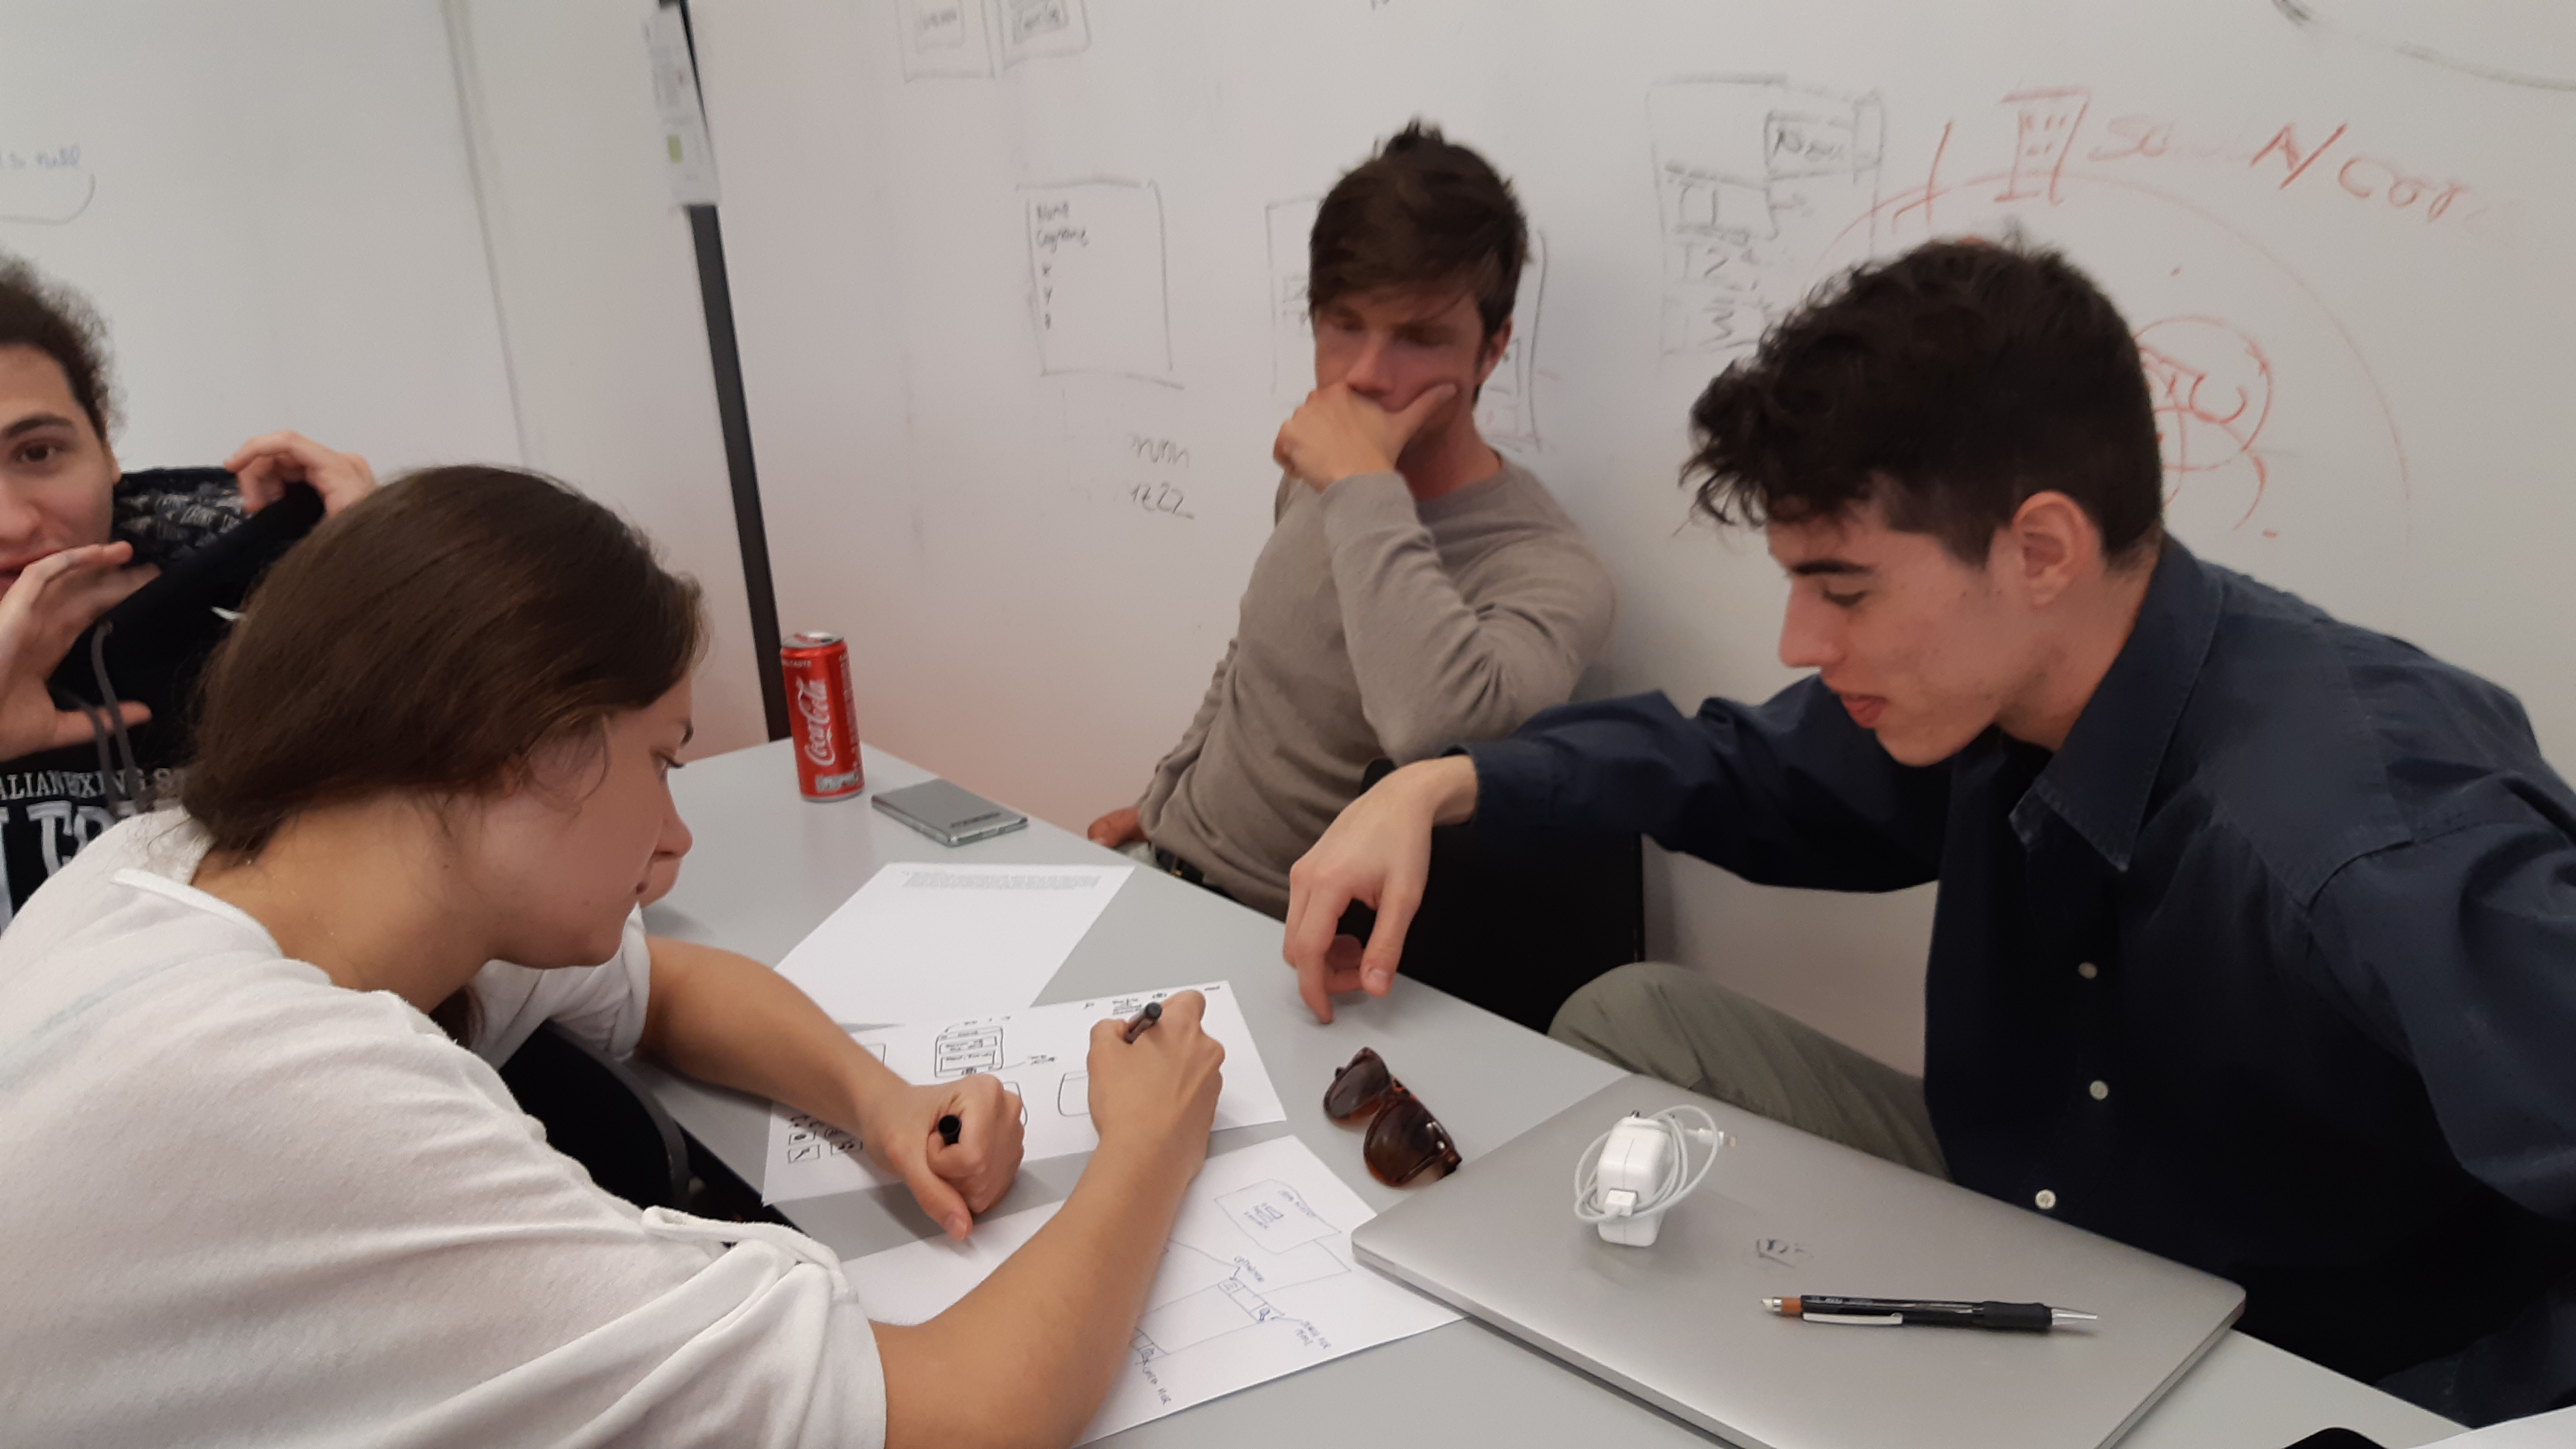
\includegraphics[width=\textwidth]{../images/group2.jpg}
       		\caption{Our team at work}
        		\label{group2}
	\end{figure}
	
	
\section{Sketches}
	
	Show scans of selected sketches.
	
	\begin{figure}[H]
        		\centering
       		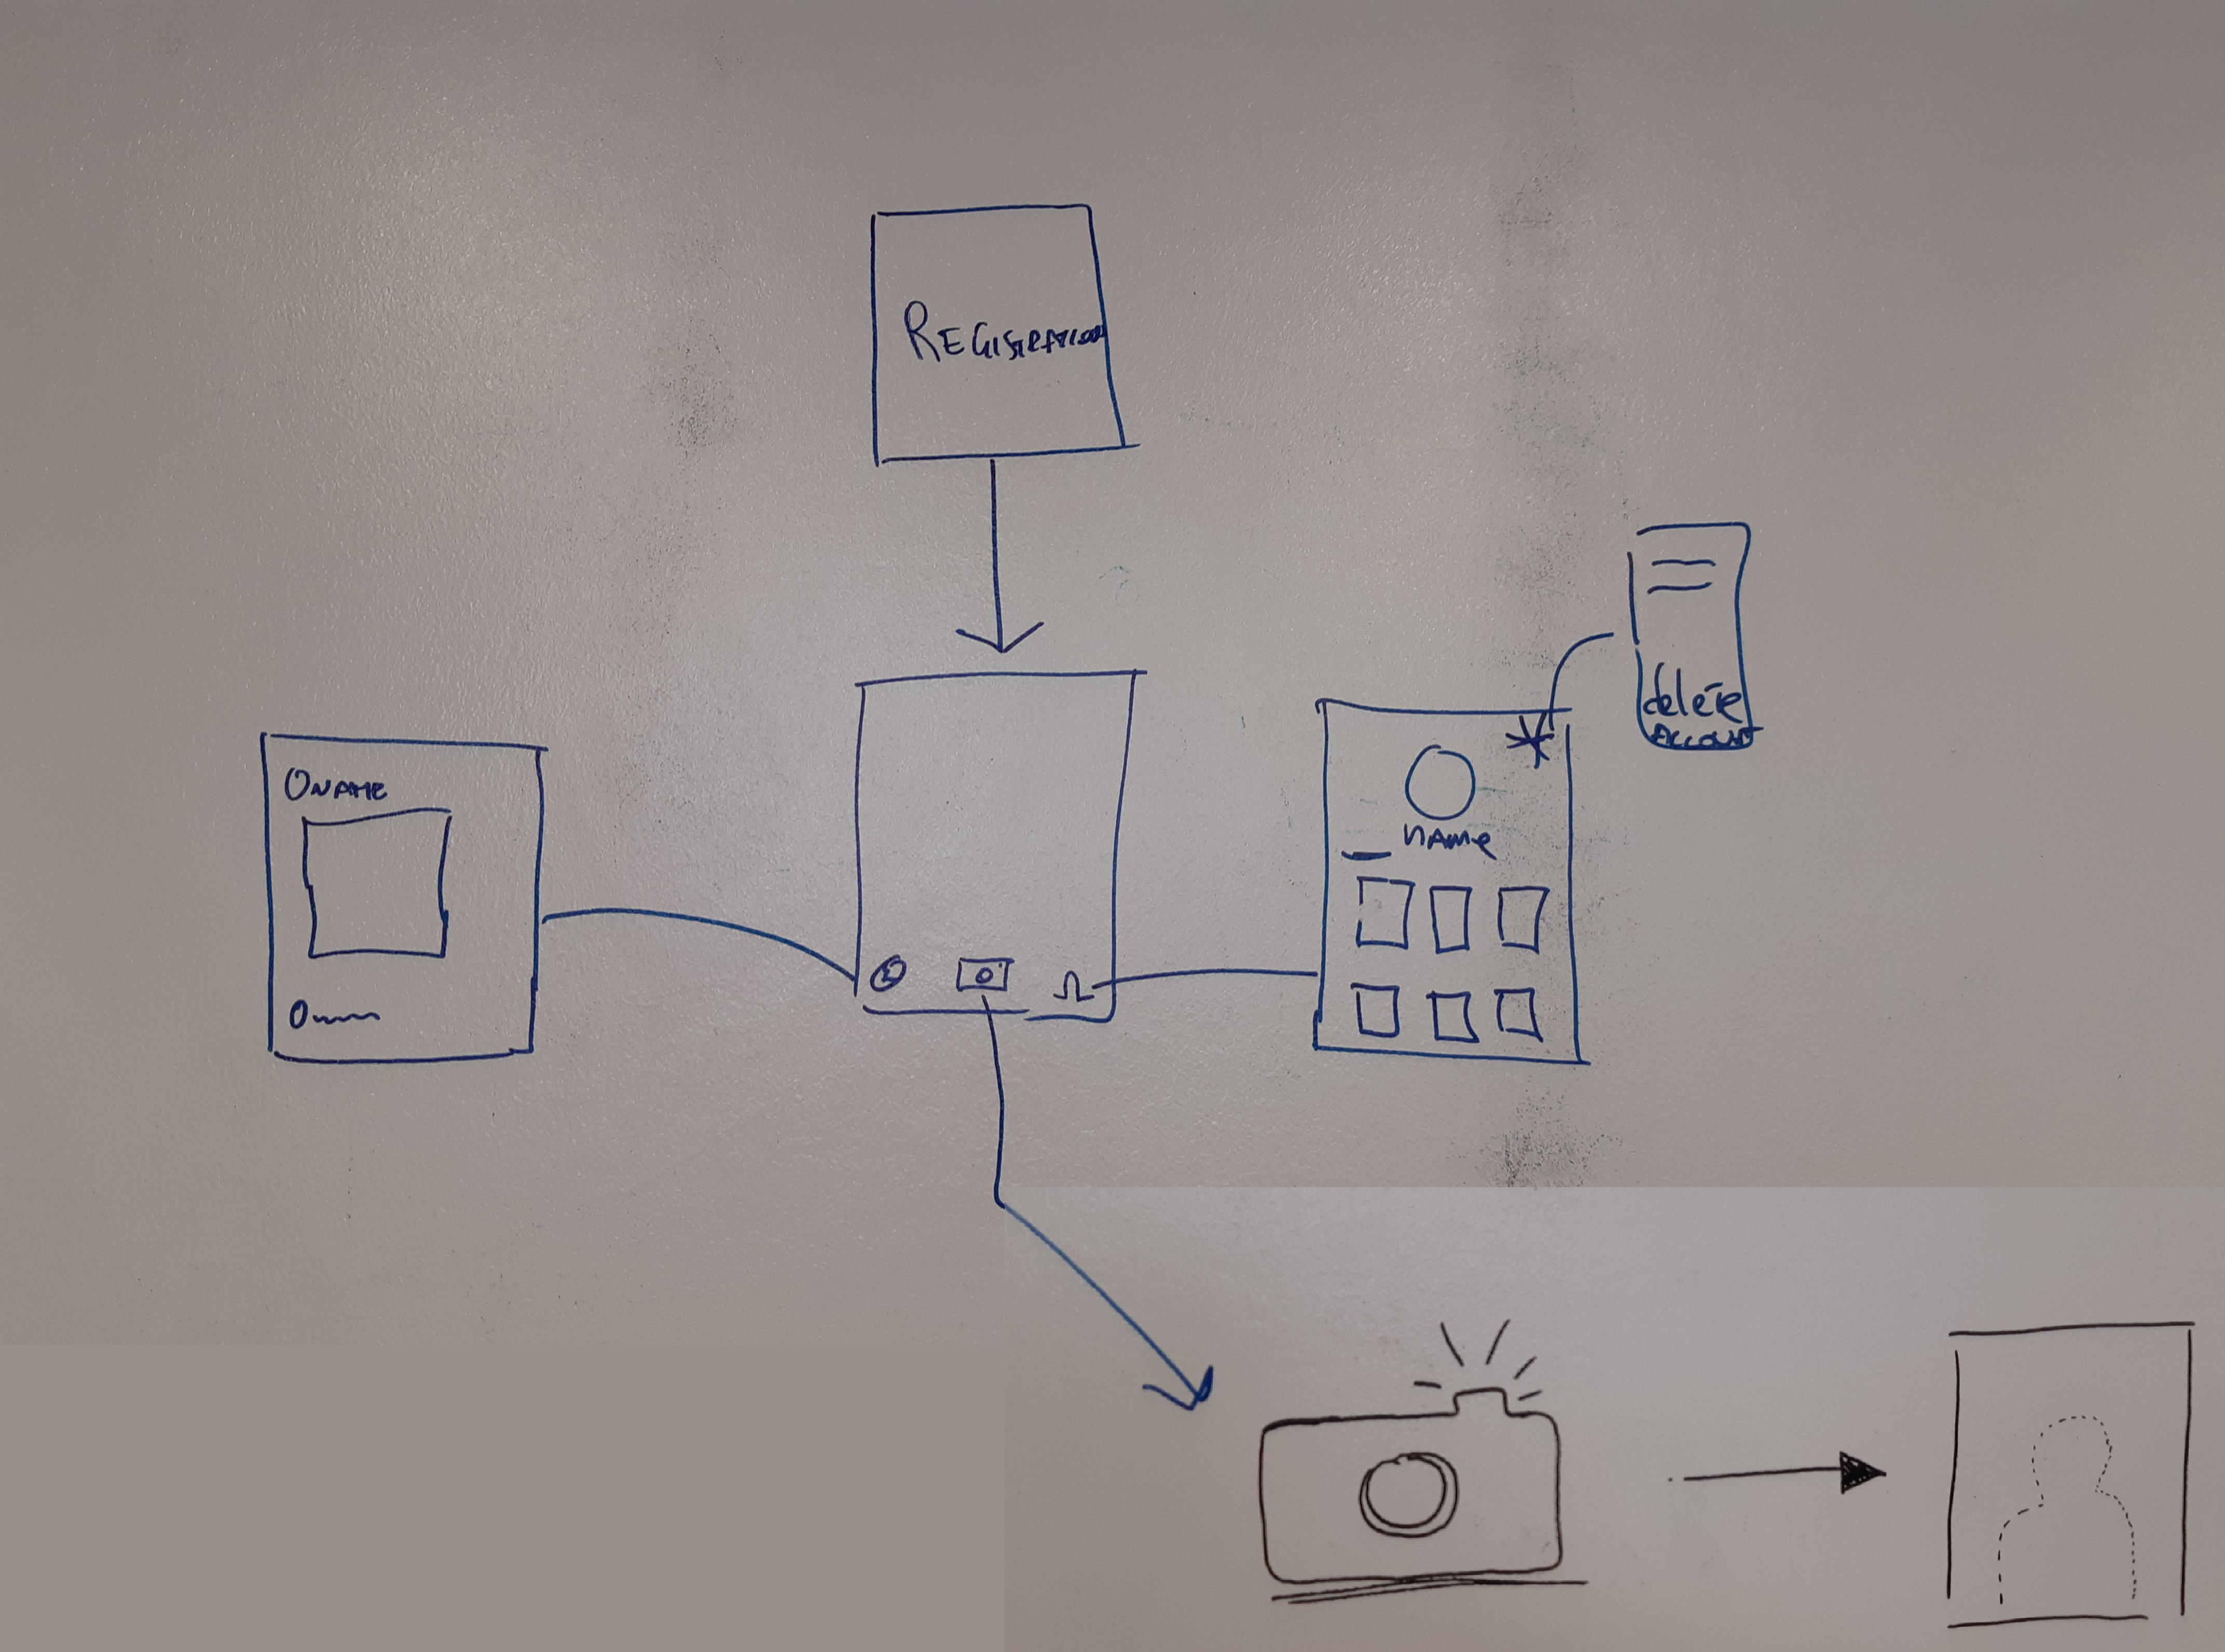
\includegraphics[width=\textwidth]{../images/design1.jpg}
       		\caption{The very first sketch}
        		\label{sketch1}
	\end{figure}
	
	\begin{figure}[H]
        		\centering
       		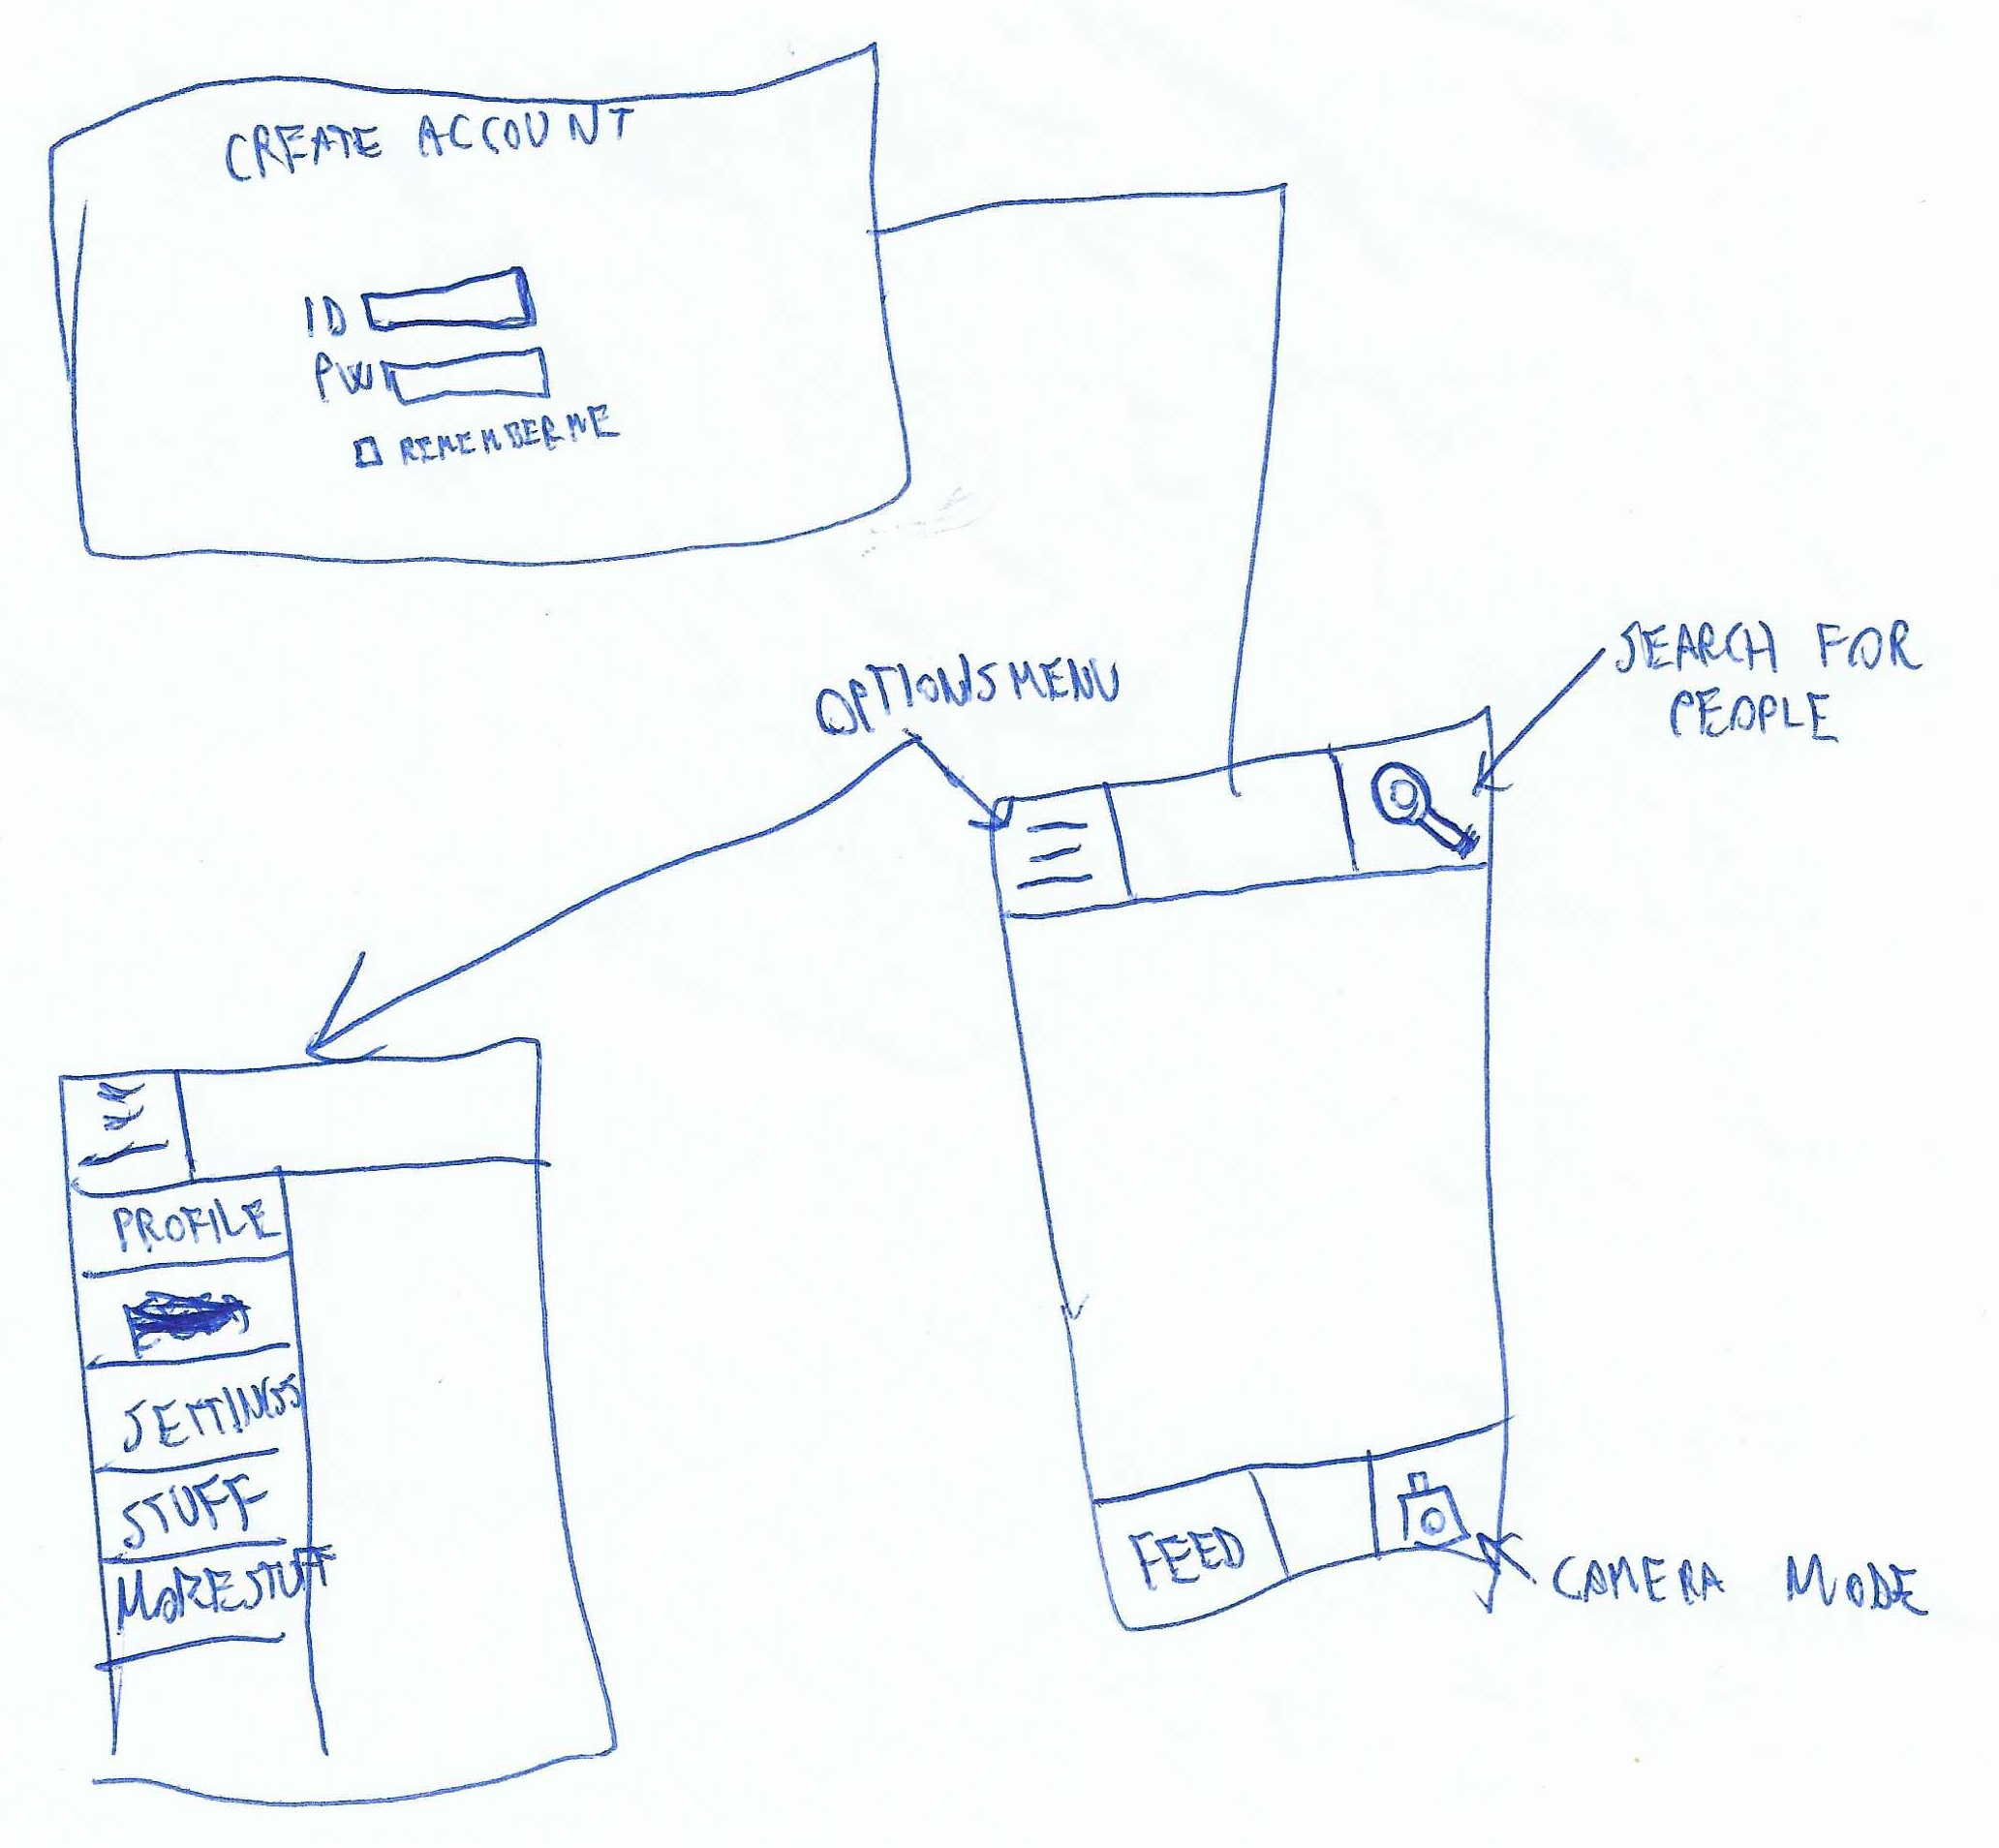
\includegraphics[width=\textwidth]{../images/design2.jpg}
       		\caption{The basic idea}
        		\label{sketch2}
	\end{figure}
	
	\begin{figure}[H]
        		\centering
       		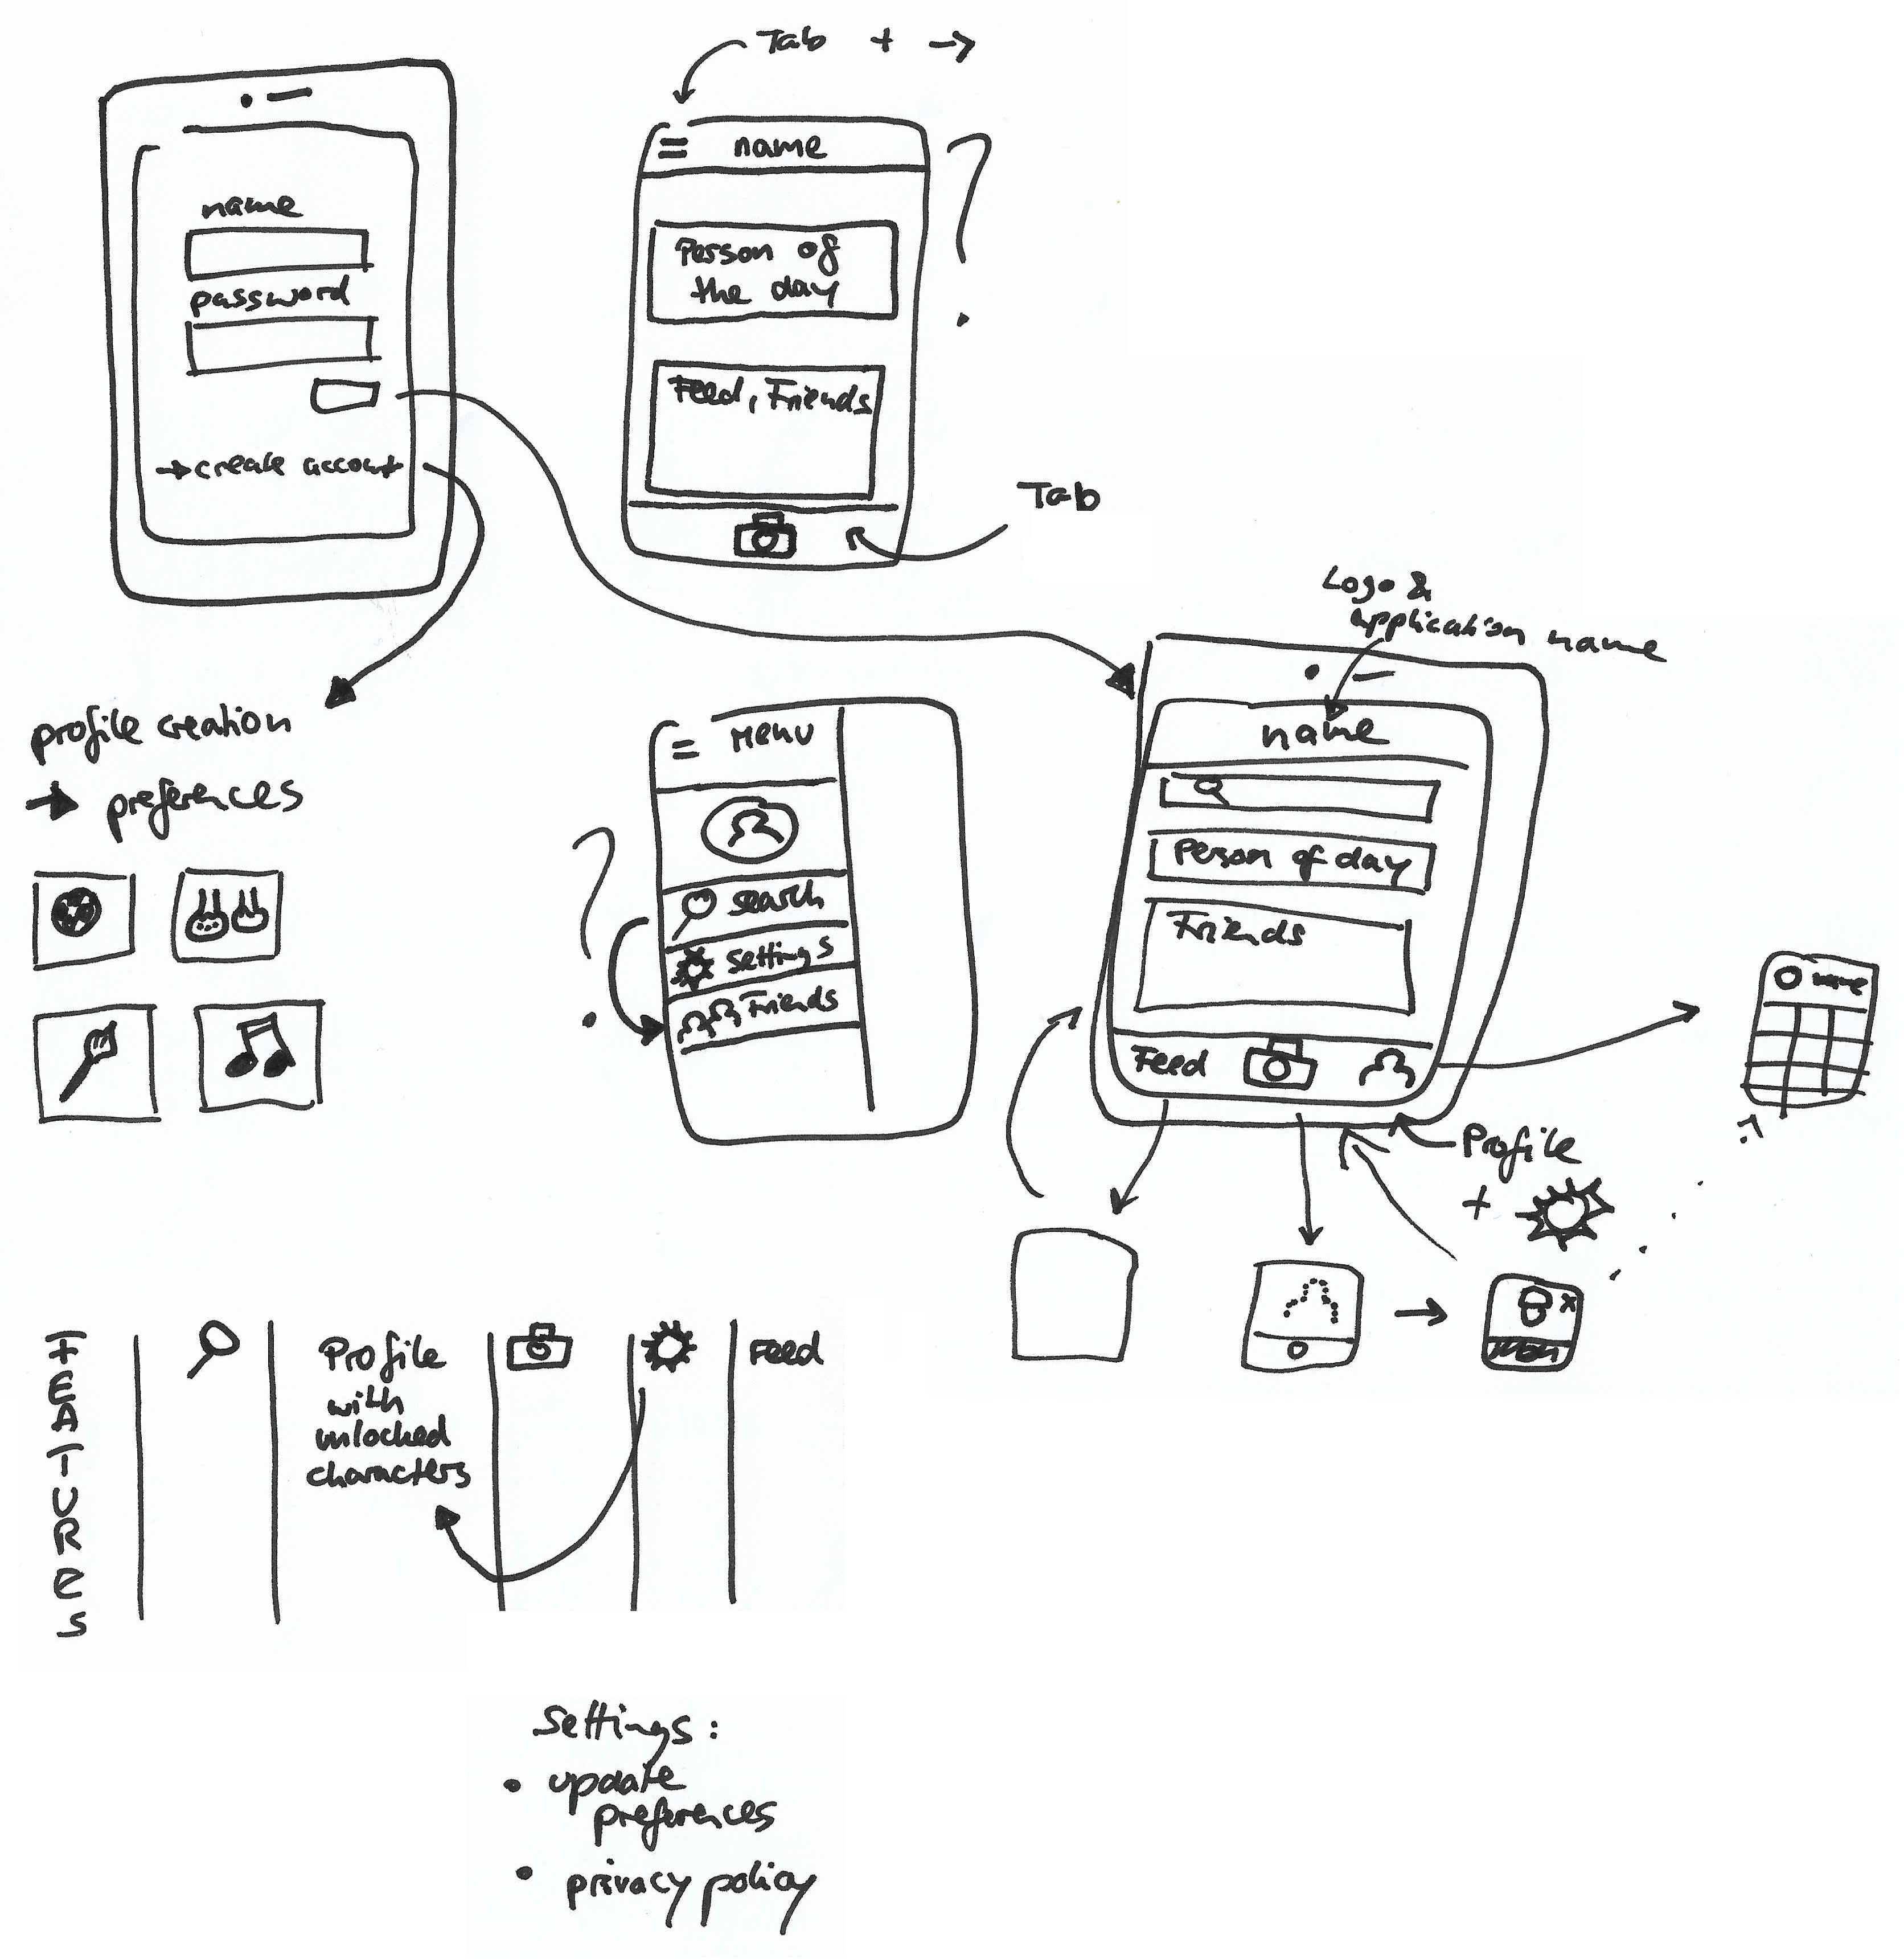
\includegraphics[width=\textwidth]{../images/design3.jpg}
       		\caption{Adding complexity}
        		\label{sketch3}
	\end{figure}
	
	
\section{Storyboard}
	
	% Show your storyboard (probably as scans or photos), and explain the process very briefly. Explain the frame that shows the transition from one adjacent frame to another.

	In this section, we will address one of the main questions behind every project, especially in application design. The question is ``why is this application useful?”. Obviously, applications are made for users and the purpose is to respond to a user need. To this end, in our application, a distinction has to be made between the user need that is satisfied and the final purpose of our application, especially that our users are children.\\

	Taking in account the fact that our users are children, our application is shaped, before all, as a game. Tendencies shows that children possessing smartphones use them mainly for playing games (Clash of Clans, Fortnite, …). That’s why we have chosen to present our application as a game, thus giving the first part of our response to the previous question. Our application is a way for children to occupy their time pleasantly.\\

	But that’s not all, as Pokémon Go did by adding in their game a touch of reality (using the camera for discovering new Pokémon), we wanted to add a touch of social dimension. Games and smartphones in general tend to hyper-connect people which can generate a social isolation. This is also true for children. That’s why our game will provide a way for the user to exchange the portrait of famous person he got with other users.\\

	This idea was inspired from cards (stickers) collections like Panini Football players and Yu-Gi-Oh!, where it is easy to observe that exchanging the famous person (which will look like a card on the application) will definitely encourage social interaction between children and avoid isolation risk. We then add a second part to our initial answer, not only will children occupy their time but our application will supposedly encourage social interaction.\\

	Now we will proceed to explain what is the final purpose of our application and why is it useful for children in term of educative purpose.\\

	The hyper-connectivity we are facing nowadays create some drawback, the first and most obvious that we experiment everyday is the astronomical quantities of information we received every day though emails, social networks, news applications, embedded notifications and so on. This drawback, although in appearance more boring than constituting a matter of concern, is in reality quite dangerous. In deed, we are influenced by all this flow of information, consciously and unconsciously. This particularly true in the sense that, often, the flow of information is constituted of ``buzz” and usually, these viral buzz are bad examples and stupidities of famous person’s everyday life. And more than us, children are influenced by these information.\\

	It is here that our application takes place, by playing with portrait of famous persons who gain their fame through noble actions (peace Nobel prize, people saving, medical and scientific discoveries, ...), children will get positively influenced by these persons. Of course, the idea is create rich and interesting descriptions, small audio and video podcast about every famous portrait in order to really invite the child to look at the information and to learn about the life of these persons. Not only are the children positively influenced, but they also learn about the history and the famous discoveries that happened in our world. This could generate center of interest and maybe, with a little luck, passion discoveries. At least, that would be the best goal our application could achieve!\\

	\textbf{Android studio}\\

	After having set up the Android Studio environment into Intellij IDEA, we have played a bit with the functionalities and we are now considering the feasibility of programming the user interface of our application with it. The next step is to follow some tutorial and check if something nice can be done with it and what would be the complexity.\\

	\begin{figure}[H]
        		\centering
       		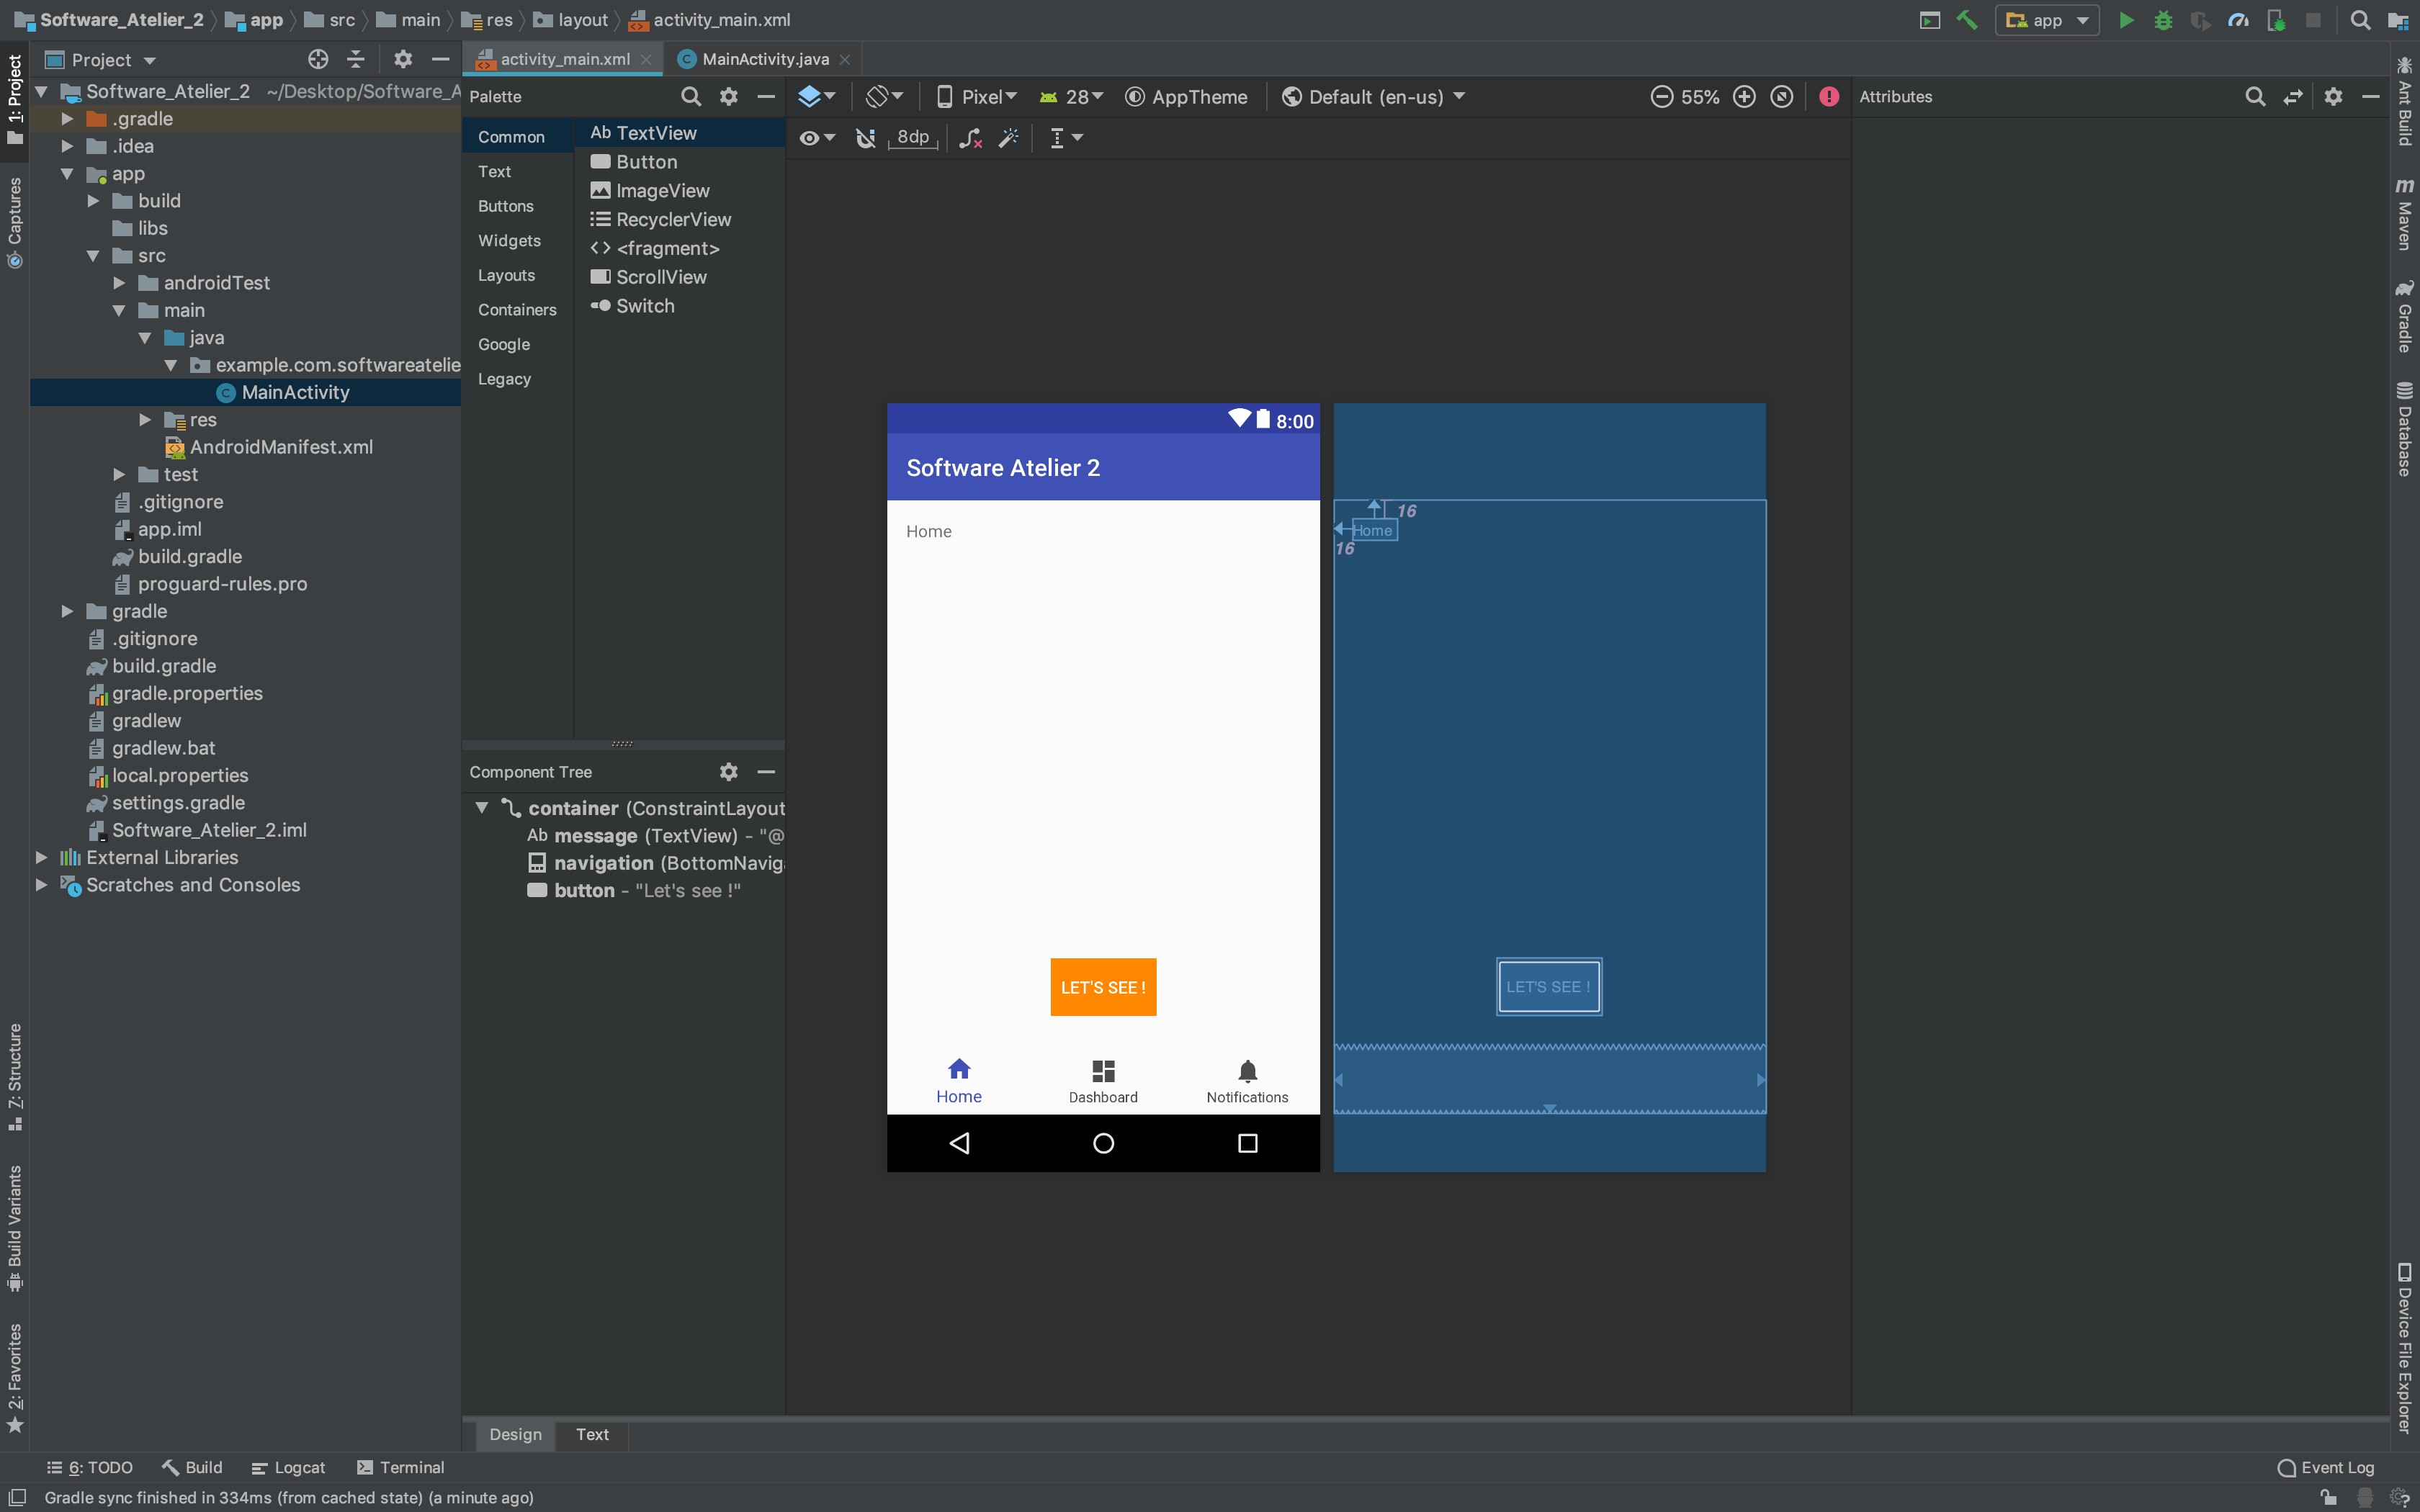
\includegraphics[width=\textwidth]{../images/androidStudio1.png}
       		\caption{The interface design in Anrdoid Studio}
        		\label{androirdStudio1}
	\end{figure}
	
	\begin{figure}[H]
        		\centering
       		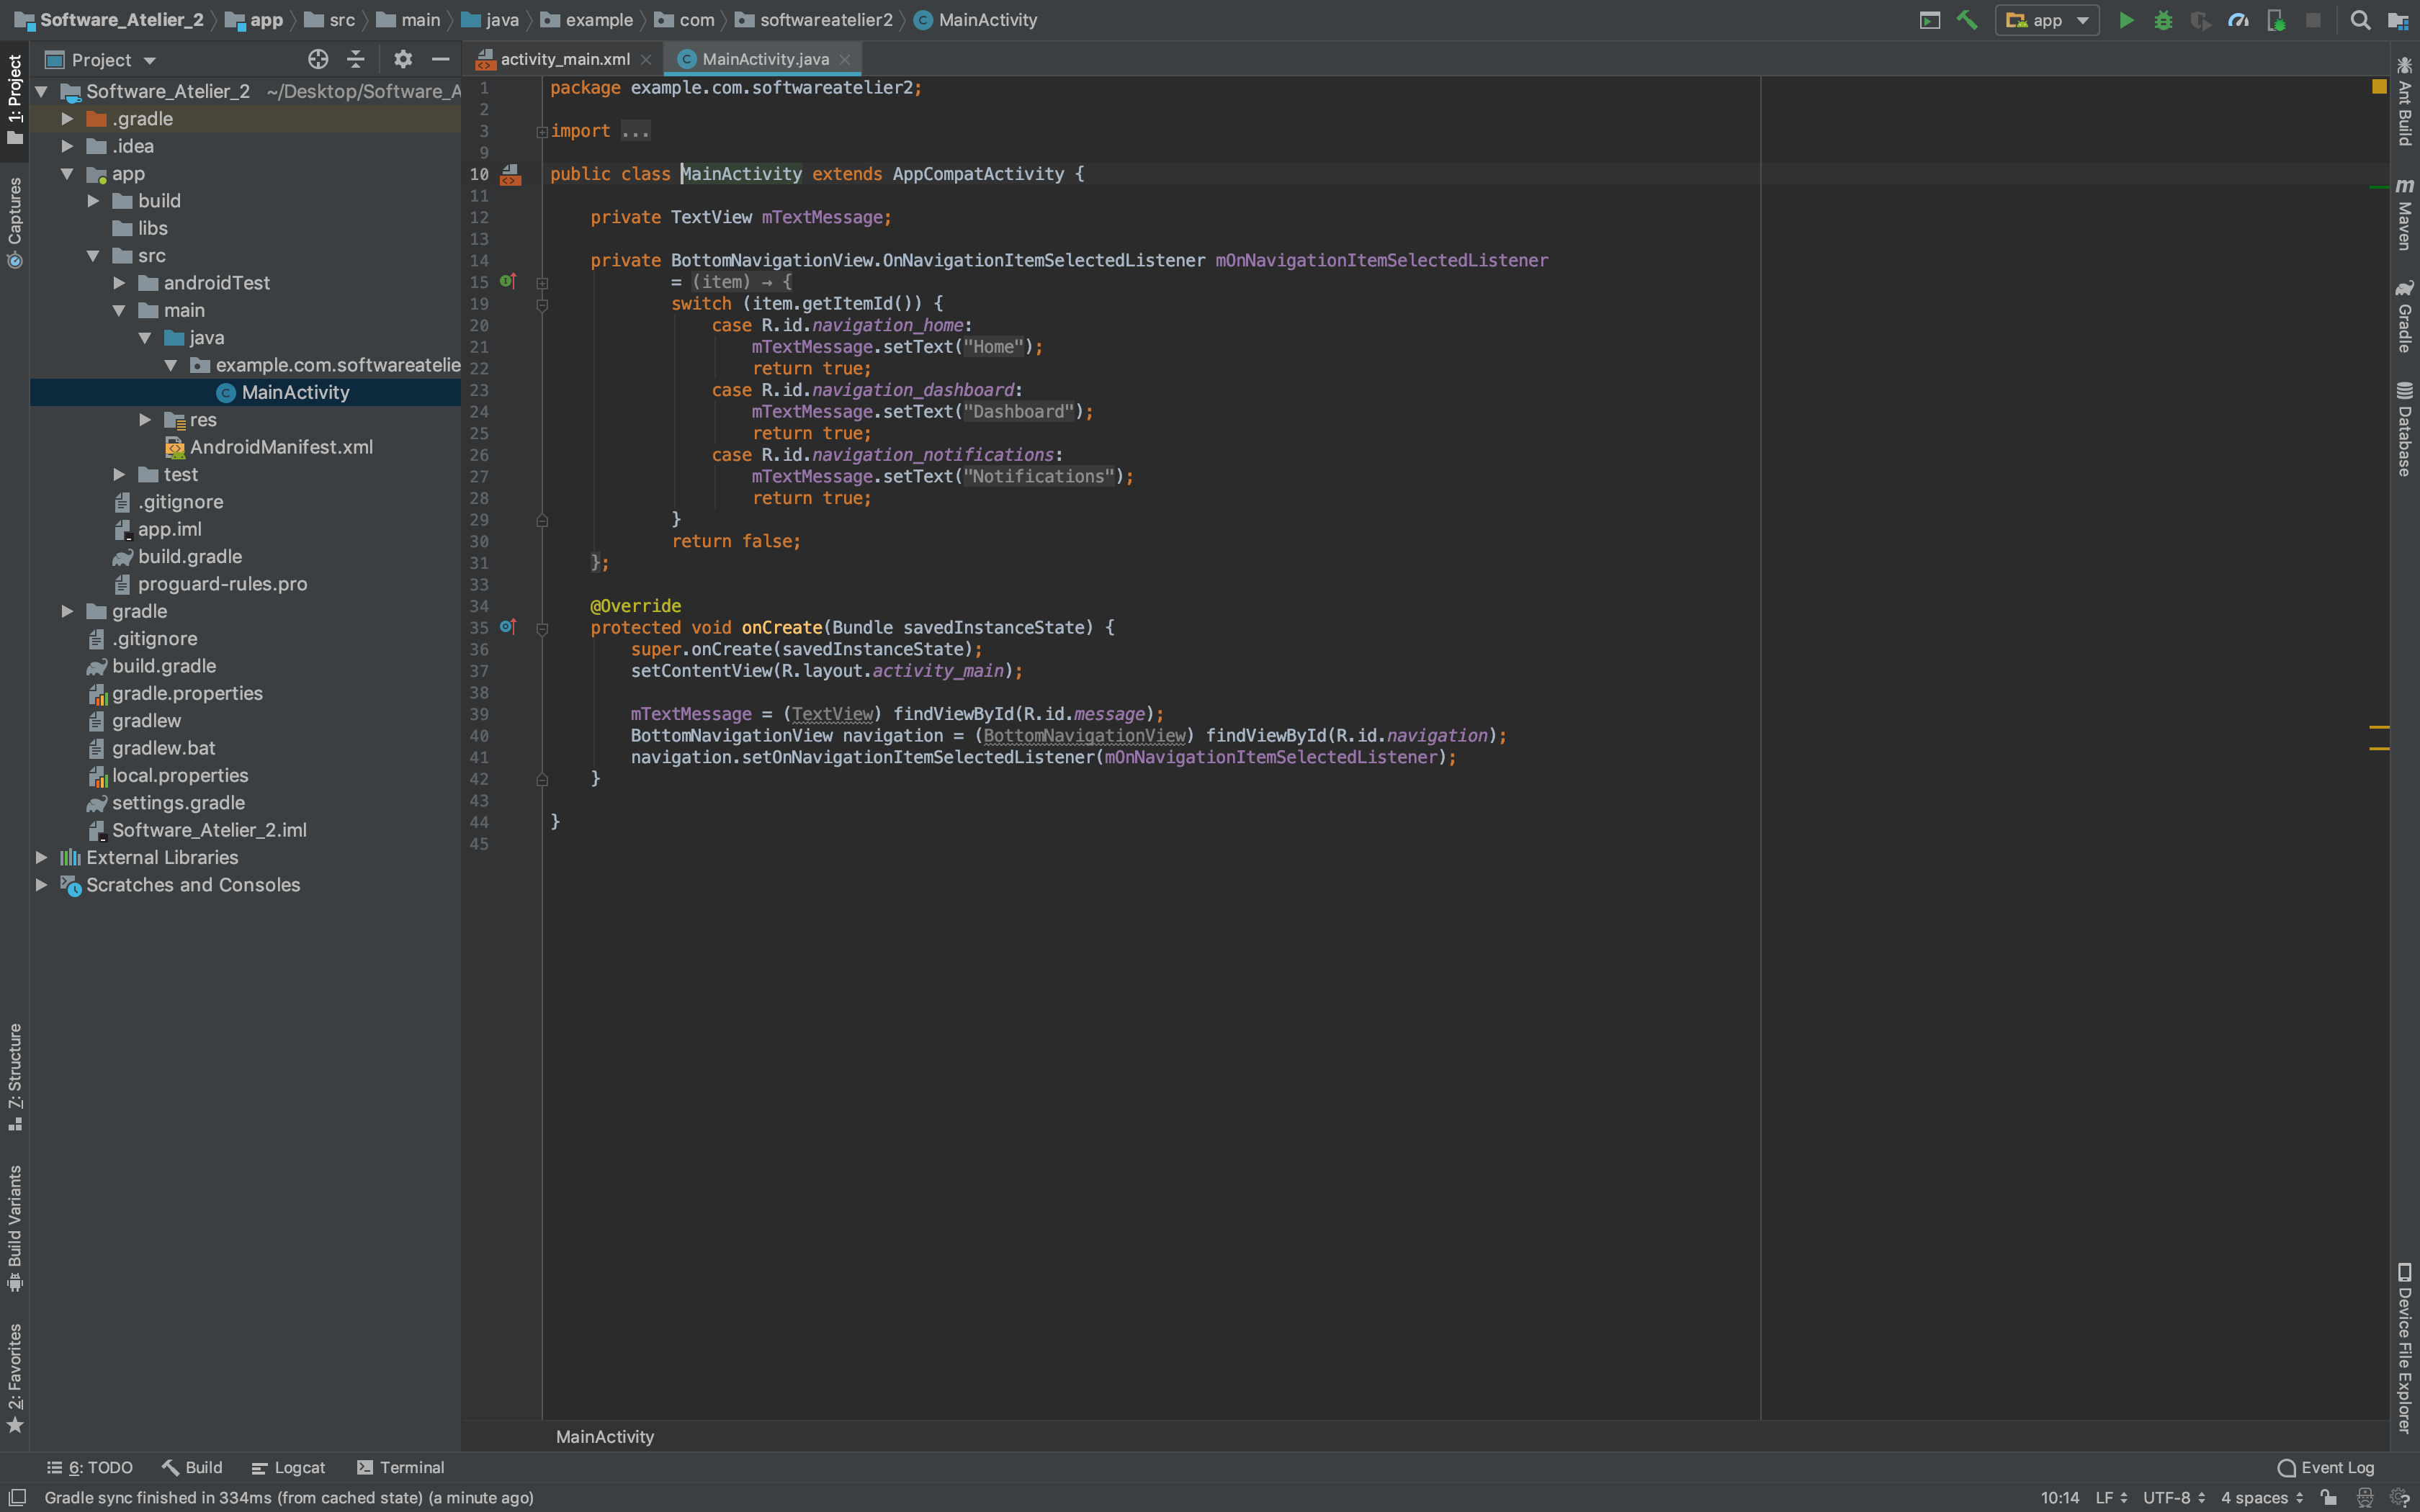
\includegraphics[width=\textwidth]{../images/androidStudio2.png}
       		\caption{The Java code behind it}
        		\label{androirdStudio2}
	\end{figure}
	
	\begin{figure}[H]
        		\centering
       		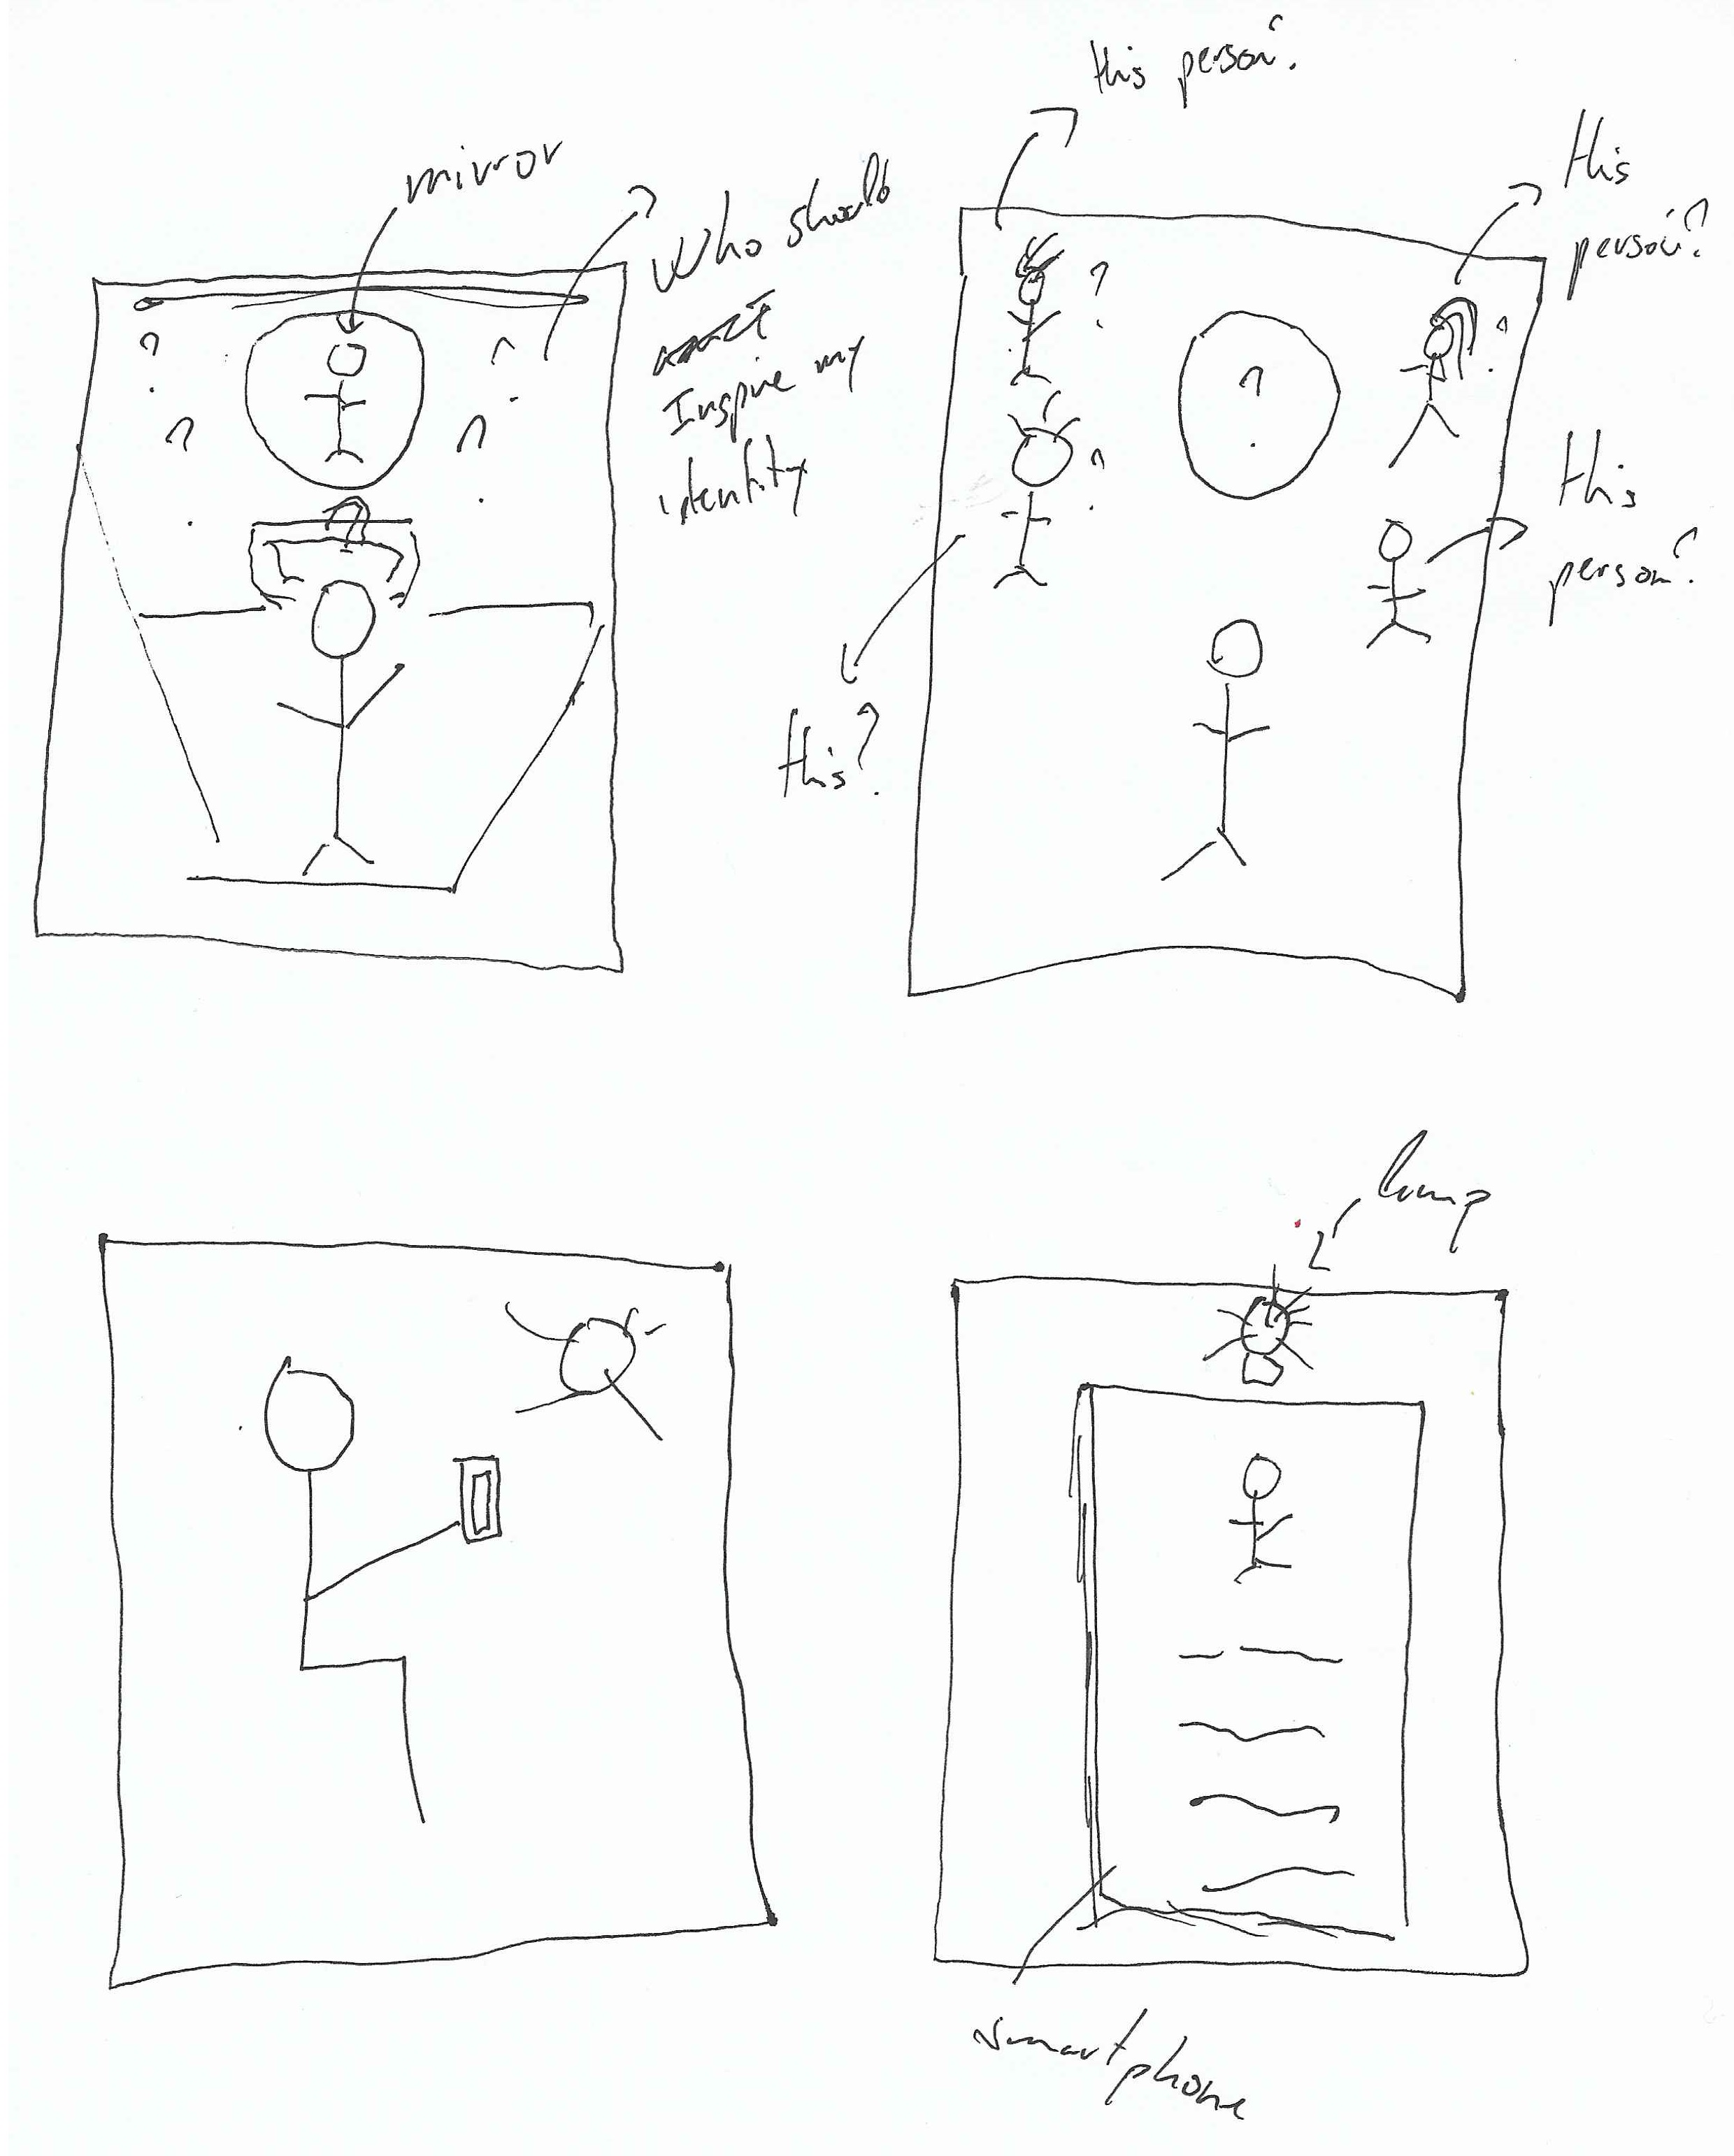
\includegraphics[width=\textwidth]{../images/story1.jpg}
       		\caption{The First Story (by Filippo)}
        		\label{story1}
	\end{figure}
	
	\begin{figure}[H]
        		\centering
       		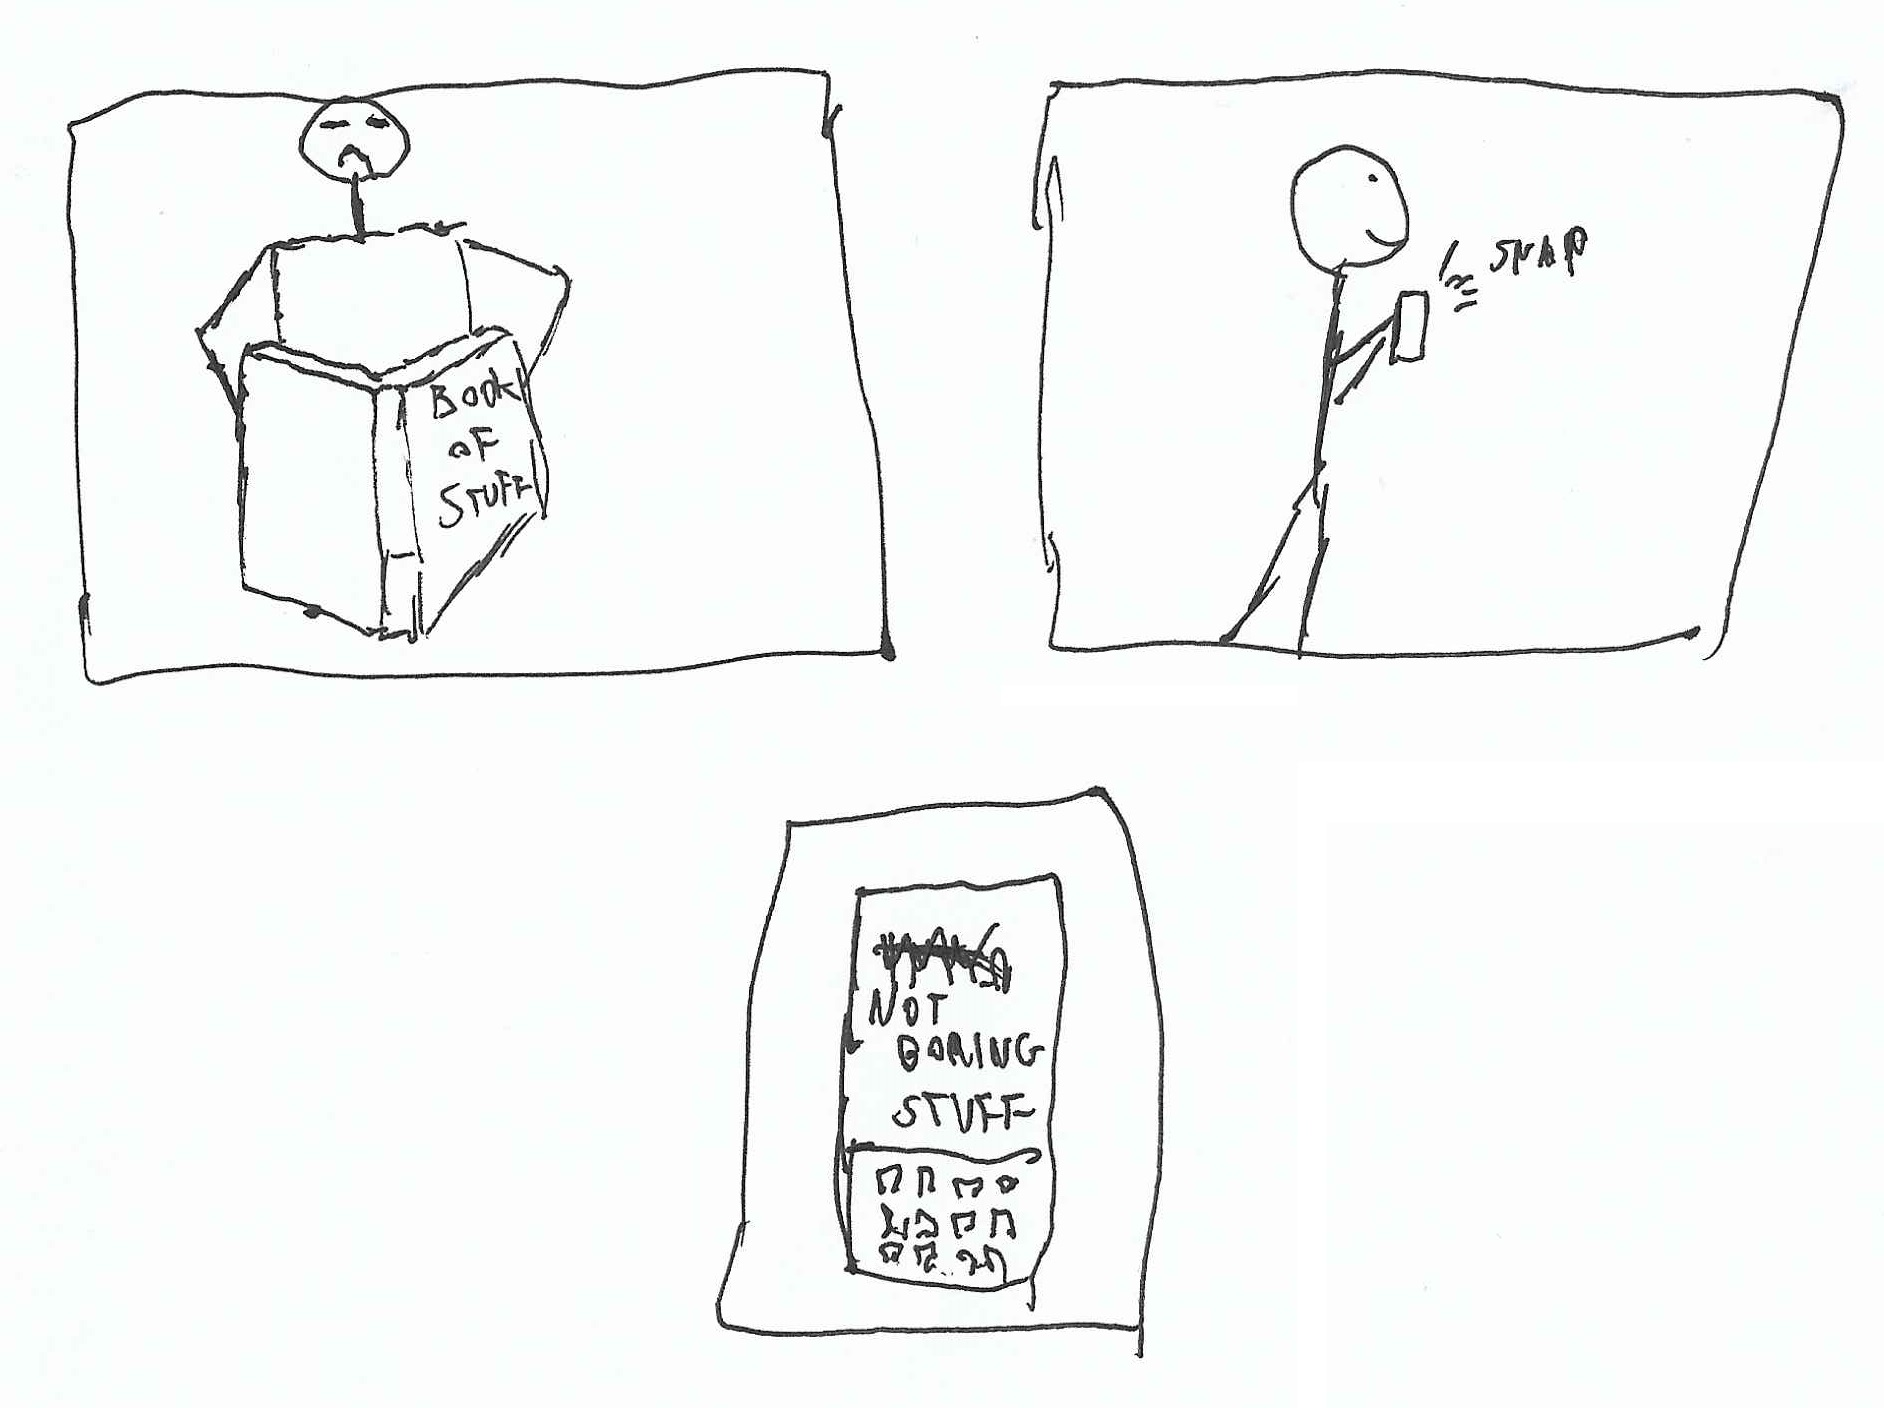
\includegraphics[width=\textwidth]{../images/story2.jpg}
       		\caption{The Second Story (by Tommaso)}
        		\label{story2}
	\end{figure}
	
	\begin{figure}[H]
        		\centering
       		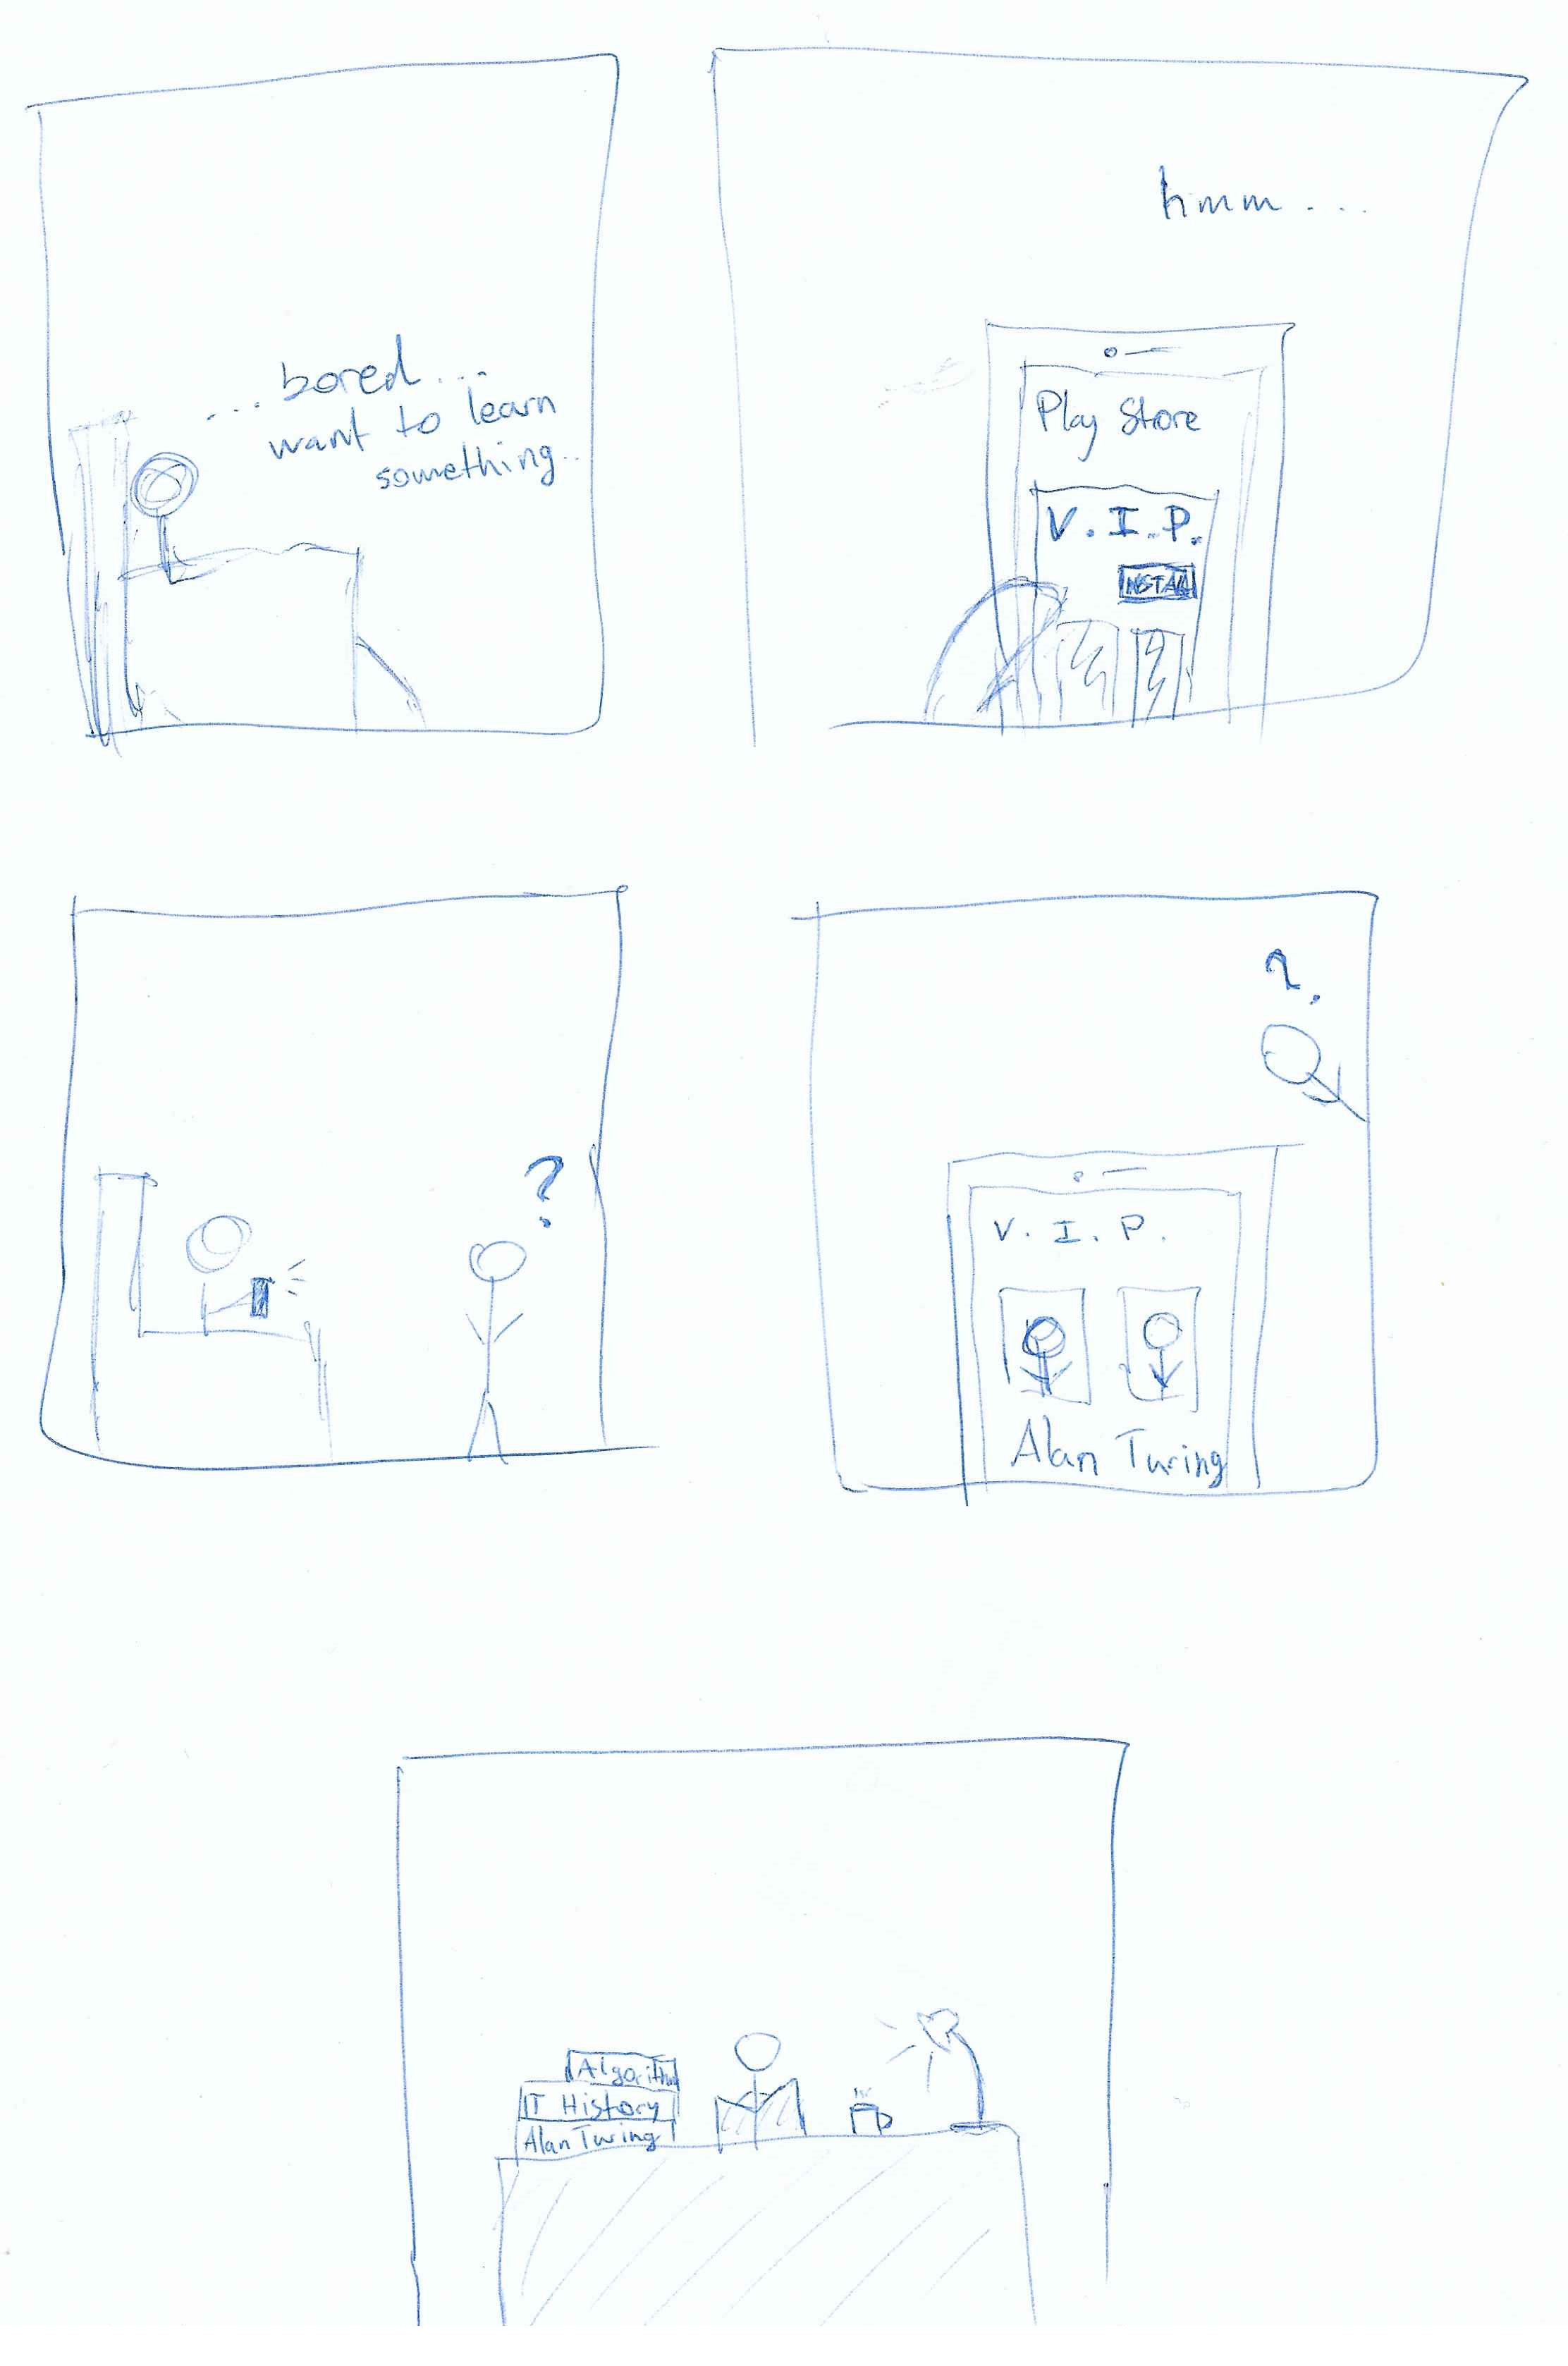
\includegraphics[width=\textwidth]{../images/story3.jpg}
       		\caption{The Third Story (by Stefano)}
        		\label{story3}
	\end{figure}
	
	\begin{figure}[H]
        		\centering
       		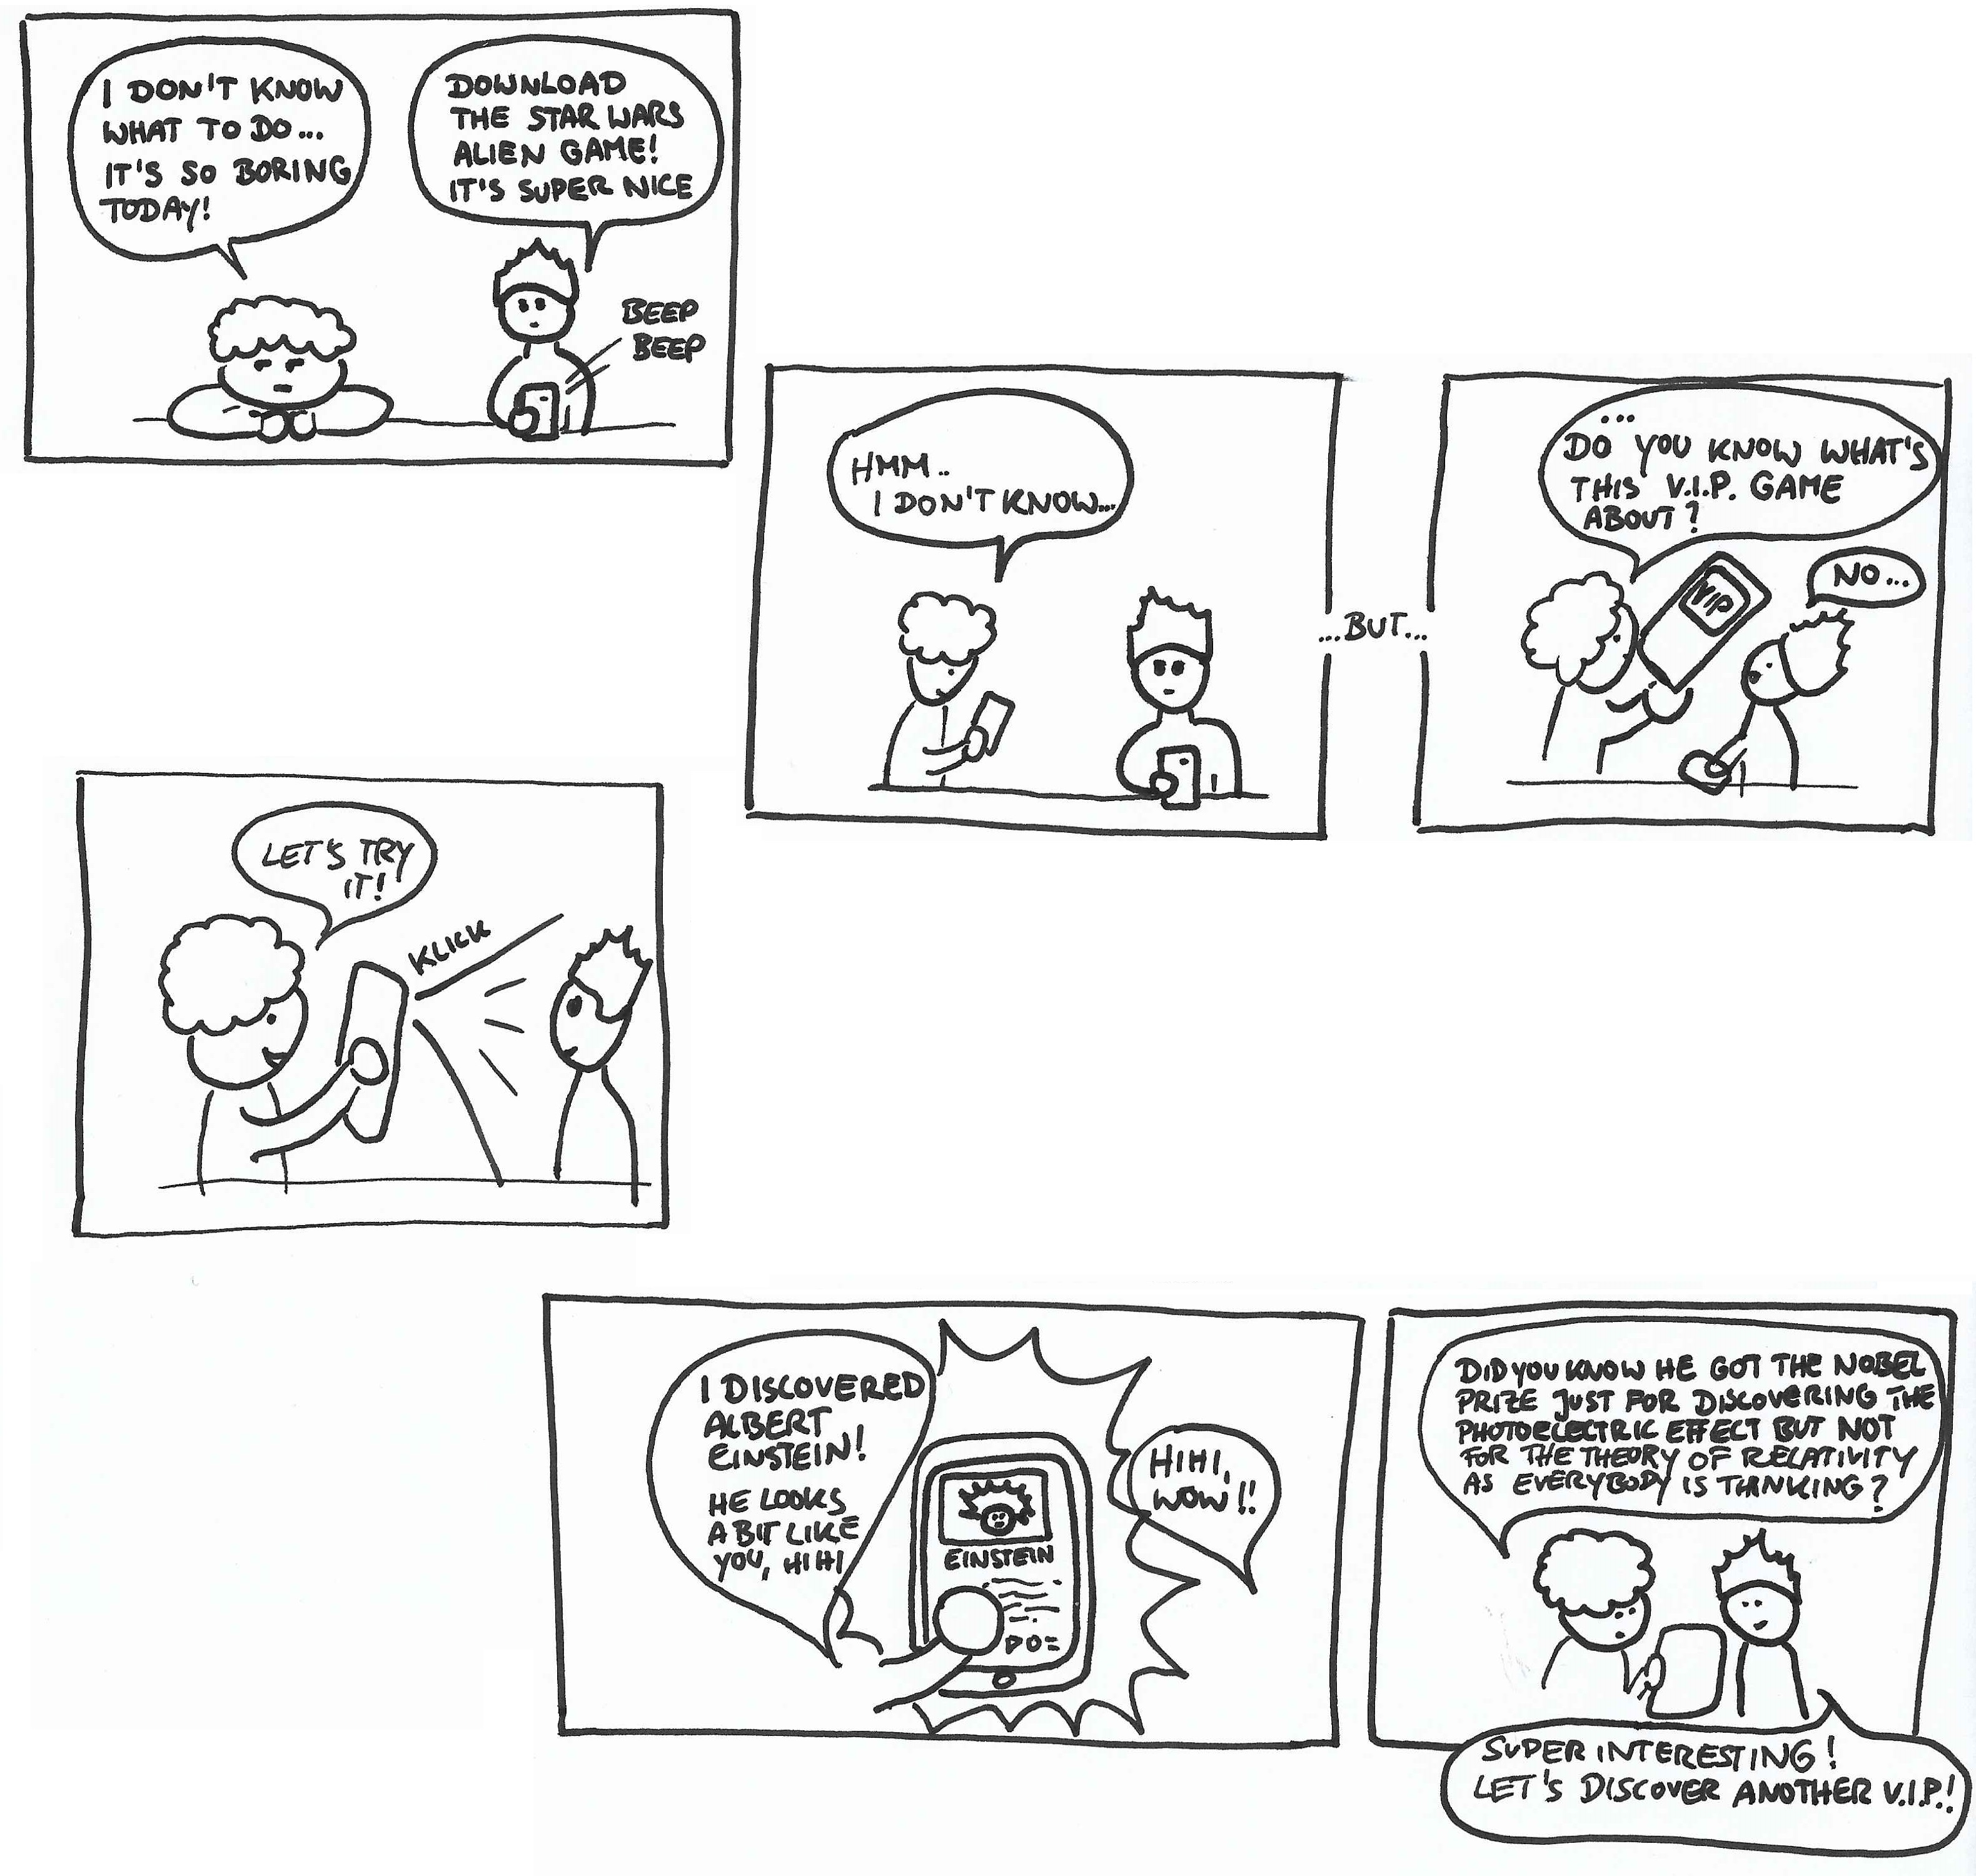
\includegraphics[width=\textwidth]{../images/story4.jpg}
       		\caption{The Fourth Story (by Kathrin)}
        		\label{story4}
	\end{figure}
	

\section{Wireframes}

	%Make a wireframe representation of a set of related intermediate screen designs, corresponding to the usage/design scenario you used for the storyboard above.  Show screen layout and navigation.
	
	\begin{figure}[H]
        		\centering
       		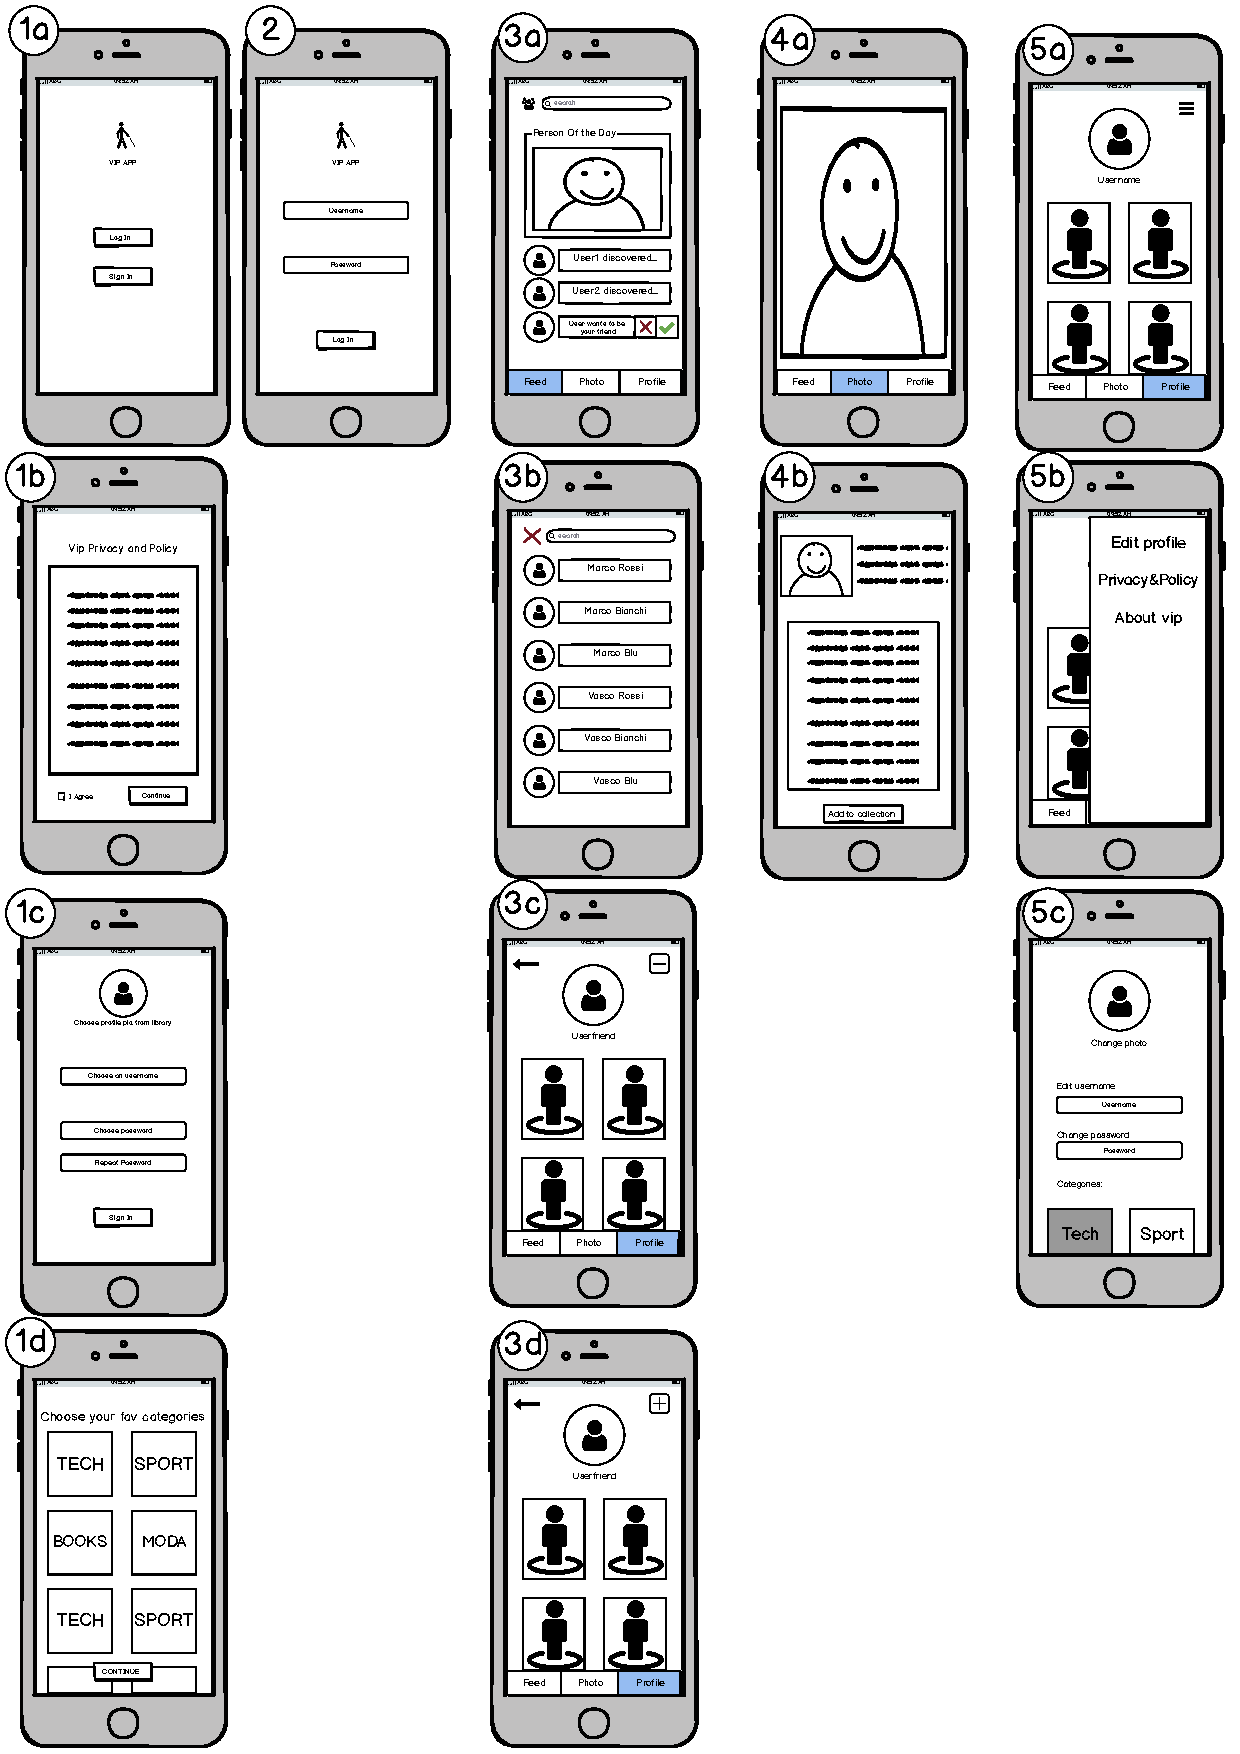
\includegraphics[width=\textwidth]{wireframes.pdf}
       		\caption{Our Balsamiq wireframes}
        		\label{wireframes}
	\end{figure}
	
	
\section{Conclusions}

	%Write conclusions about what you have learned and progress in your project.
	
	To summarize, after having had the basic idea, our first goal was to define the persona of our app. This challenge has been overcome by interviewing young people with an age around 12 years old, who, we thought, could have represented a good benchmark to frame our possible community. While at the beginning we thought that it could have been difficult to obtain the answers we were looking for, thus remaining with an unclear idea of our users preferences and interest when it comes to social apps, we then discovered that the you people we interviewed were very talking active and interested in sharing their digital ideas and smartphone habits. Even though our app can be enjoyed at every age and by any cultural background, these interviews were fundamental to determine more precisely our persona; and after having synthesized the data, we had a defined picture of our possible users.\\
	
	Once we understood which creative direction our app would have taken, we worked at the app presentation, that is how quickly and entertaining transmit to the public our app concept. To do this, we used sketches and storyboards. Since every app is easier to sell when it solves a problem, our goal was to translate the app usage in terms of daily life challenges to overcome. Once it was apparent for which difficulty our app can be useful, we had to create a story in which the user could identify herself.\\
  
	Our last task was to actually design the graphic user interface. This creative job was facilitated by the use of Balsamiq, which is a helpful online tool to create wireframes and to quickly look at the possible final product. Since nothing is more useful than studying and learning from already successful apps similar to the one you are developing, we looked closely at the Instagram GUI, thus enhancing our chances to be appealing and already familiar to our users. \\
  
	In conclusion, developing an app is a process which, on the one hand, must be approached by a team who is able to assign different task to different team members, working at the same time together and individually, but always following the same project goals. On the other hand, the creation of an app must be divided in sub-creative tasks, such as the study of the persona, of the wireframes, etc. which ultimately make it easier to avoid risks, be efficient, and probably producing a high-quality product which hopefully could reach a vast audience.	

\end{document}